\documentclass[a4paper]{article}

%------------------------------------------------------------
\usepackage[a4paper, total={6in, 9in}]{geometry}
\usepackage{amsmath, amssymb}
\usepackage{booktabs}
\usepackage{caption}
\usepackage{enumitem}
\usepackage{graphicx}
\usepackage{float}
\usepackage{inconsolata}
\usepackage{listings}
\usepackage{mathtools}
\usepackage{pstricks-add}
\usepackage{siunitx}
\usepackage[most]{tcolorbox}
\usepackage{tikz, pgfplots}
\usepackage{epstopdf} %converting to PDF
\usepackage{hyperref}
\usepackage{xfrac}

\usetikzlibrary{shapes.geometric}
\usetikzlibrary{arrows}
\usetikzlibrary{calc}

%------------------------------------------------------------
\graphicspath{{./fig/}}
\pgfplotsset{compat=1.13}
%------------------------------------------------------------
\setlength{\parindent}{0in}

\lstdefinestyle{C++}{
	language=C++,
	basicstyle=\ttfamily,
	keywordstyle=\color{blue}\ttfamily,
	stringstyle=\color{red}\ttfamily,
	commentstyle=\color{green}\ttfamily,
	morecomment=[l][\color{magenta}]{\#},
	showstringspaces=false
}

%------------------------------------------------------------
\newtcblisting[auto counter]{sexylisting}[2][]{sharp corners, 
    fonttitle=\bfseries, colframe=gray, listing only, 
    listing options={basicstyle=\ttfamily,language=C++}, 
    title=Listing \thetcbcounter: #2, #1}

%------------------------------------------------------------
\lstset{language=C++,
        basicstyle=\ttfamily,
        keywordstyle=\color{blue}\ttfamily,
        stringstyle=\color{red}\ttfamily,
        commentstyle=\color{green}\ttfamily,
        morecomment=[l][\color{magenta}]{\#},
        showstringspaces=false
}
%------------------------------------------------------------
\tikzstyle{block} = [draw, fill=blue!20, rectangle, 
    minimum height=3em, minimum width=3em]
\tikzstyle{sum} = [draw, fill=blue!20, circle, node distance=1cm]
\tikzstyle{input} = [coordinate]
\tikzstyle{output} = [coordinate]
\tikzstyle{pinstyle} = [pin edge={to-,thin,black}]

%------------------------------------------------------------
\newlength{\arrow}
\settowidth{\arrow}{\scriptsize$1000$}

\newcommand*{\myrightarrow}[1]{\xrightarrow{\mathmakebox[\arrow]{#1}}}

\newcommand{\uvec}[1]{\boldsymbol{\hat{\textbf{#1}}}}

%------------------------------------------------------------

\begin{document}
\title{ENG252 Dynamics: Project}
\author{Shane Reynolds}
\maketitle

\section{Introduction and Scope}
Torsional springs are capable of storing energy if they are displaced by some angle $\theta$ beyond their resting position. Letting $V_s$ be the energy stored in a torsional spring, and letting $\kappa$ be the torsional spring coefficient, Giancoli \cite{Giancoli:2000} defines the stored energy in a torsional spring as:
\begin{equation}
	V_s = \frac{1}{2} \kappa \theta^2
\end{equation}

The scope of this assignment is to use the stored energy in a mousetrap to move a wheeled vehicle 4.5$\si{\meter}$, deposit a load, and then travel back to the stating point.

\section{Design}
Basic strategy for vehicle mechanical operation was informed through online research - the most popular approach seemed to be a lever arm attached to the mousetrap. The lever arm is used to apply a moment to the drive shaft via the string, causing the wheels to turn as the mousetrap is de-energised. The overall vehicle construction can be seen in Figure 1. Figures 2 and 3 show a detailed view of the string wound onto the drive shaft; and the mousetrap with attached lever arm, respectively. The main alteration to researched designs involved attaching buffers to the drive shaft. This allowed for an increase in drive shaft torque on take off for both initial and return legs of vehicle excursion. Increased torque provides greater angular acceleration, which translates to increased linear acceleration. The string is wound such that once vehicle velocity is sufficient the string shifts back to the shaft ensuring enough rotation to traverse the required distance.

\begin{figure}[h]
	\centering
	\begin{minipage}{0.45\textwidth}
		\centering
		\frame{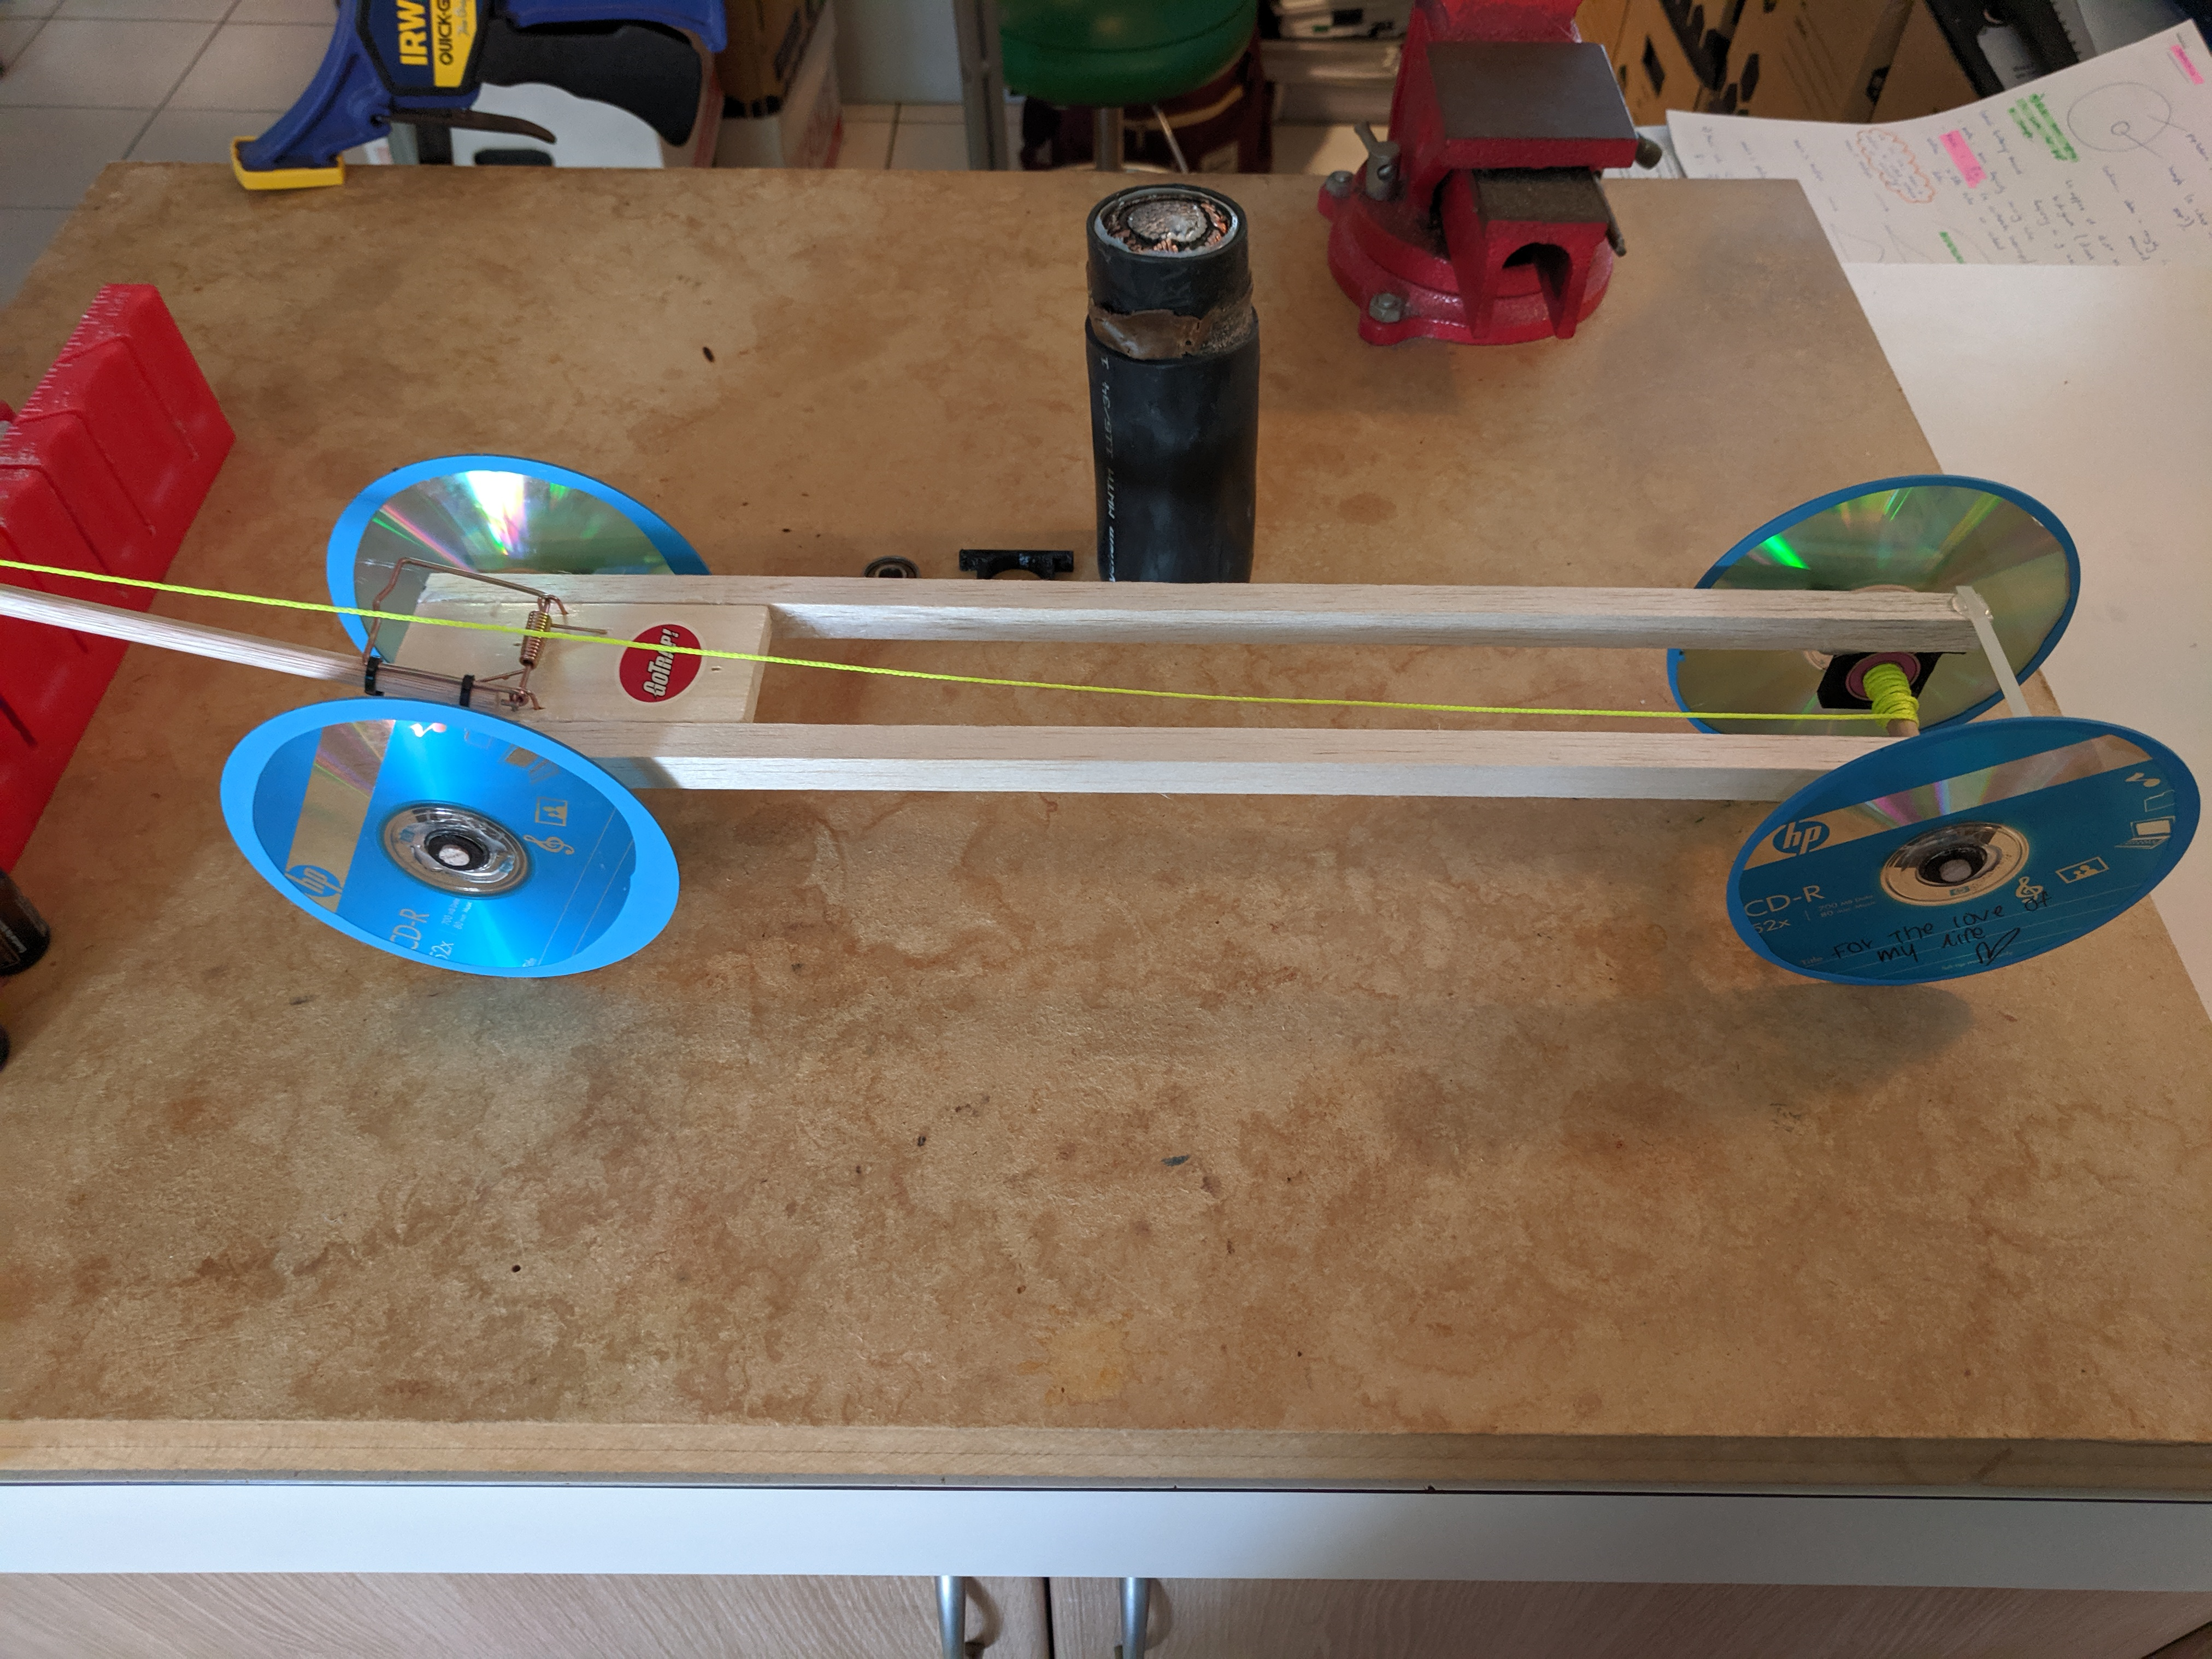
\includegraphics[height=5cm]{car}}
		\caption{The vehicle is powered by the torsional spring in the mousetrap. A lever arm is attached to the mousetrap which applies a moment to the drive shaft via the string.}
	\end{minipage}
	\hspace{1cm}
	\begin{minipage}{0.45\textwidth}
		\centering
		\captionof{table}{Key vehicle characteristics.}
		\begin{tabular}{p{3cm}rc}
			\toprule
			Measurement & Value & Unit \\
			\midrule
			Chassis Length & & \\
			Chassis Width & & \\
			Chassis Height & & \\
			Mass & 0.180 & $\si{\kilogram}$ \\
			\bottomrule
		\end{tabular}
	\end{minipage}	
\end{figure}

\begin{figure}[h]
	\centering
	\begin{minipage}[t]{0.45\textwidth}
		\centering
		\frame{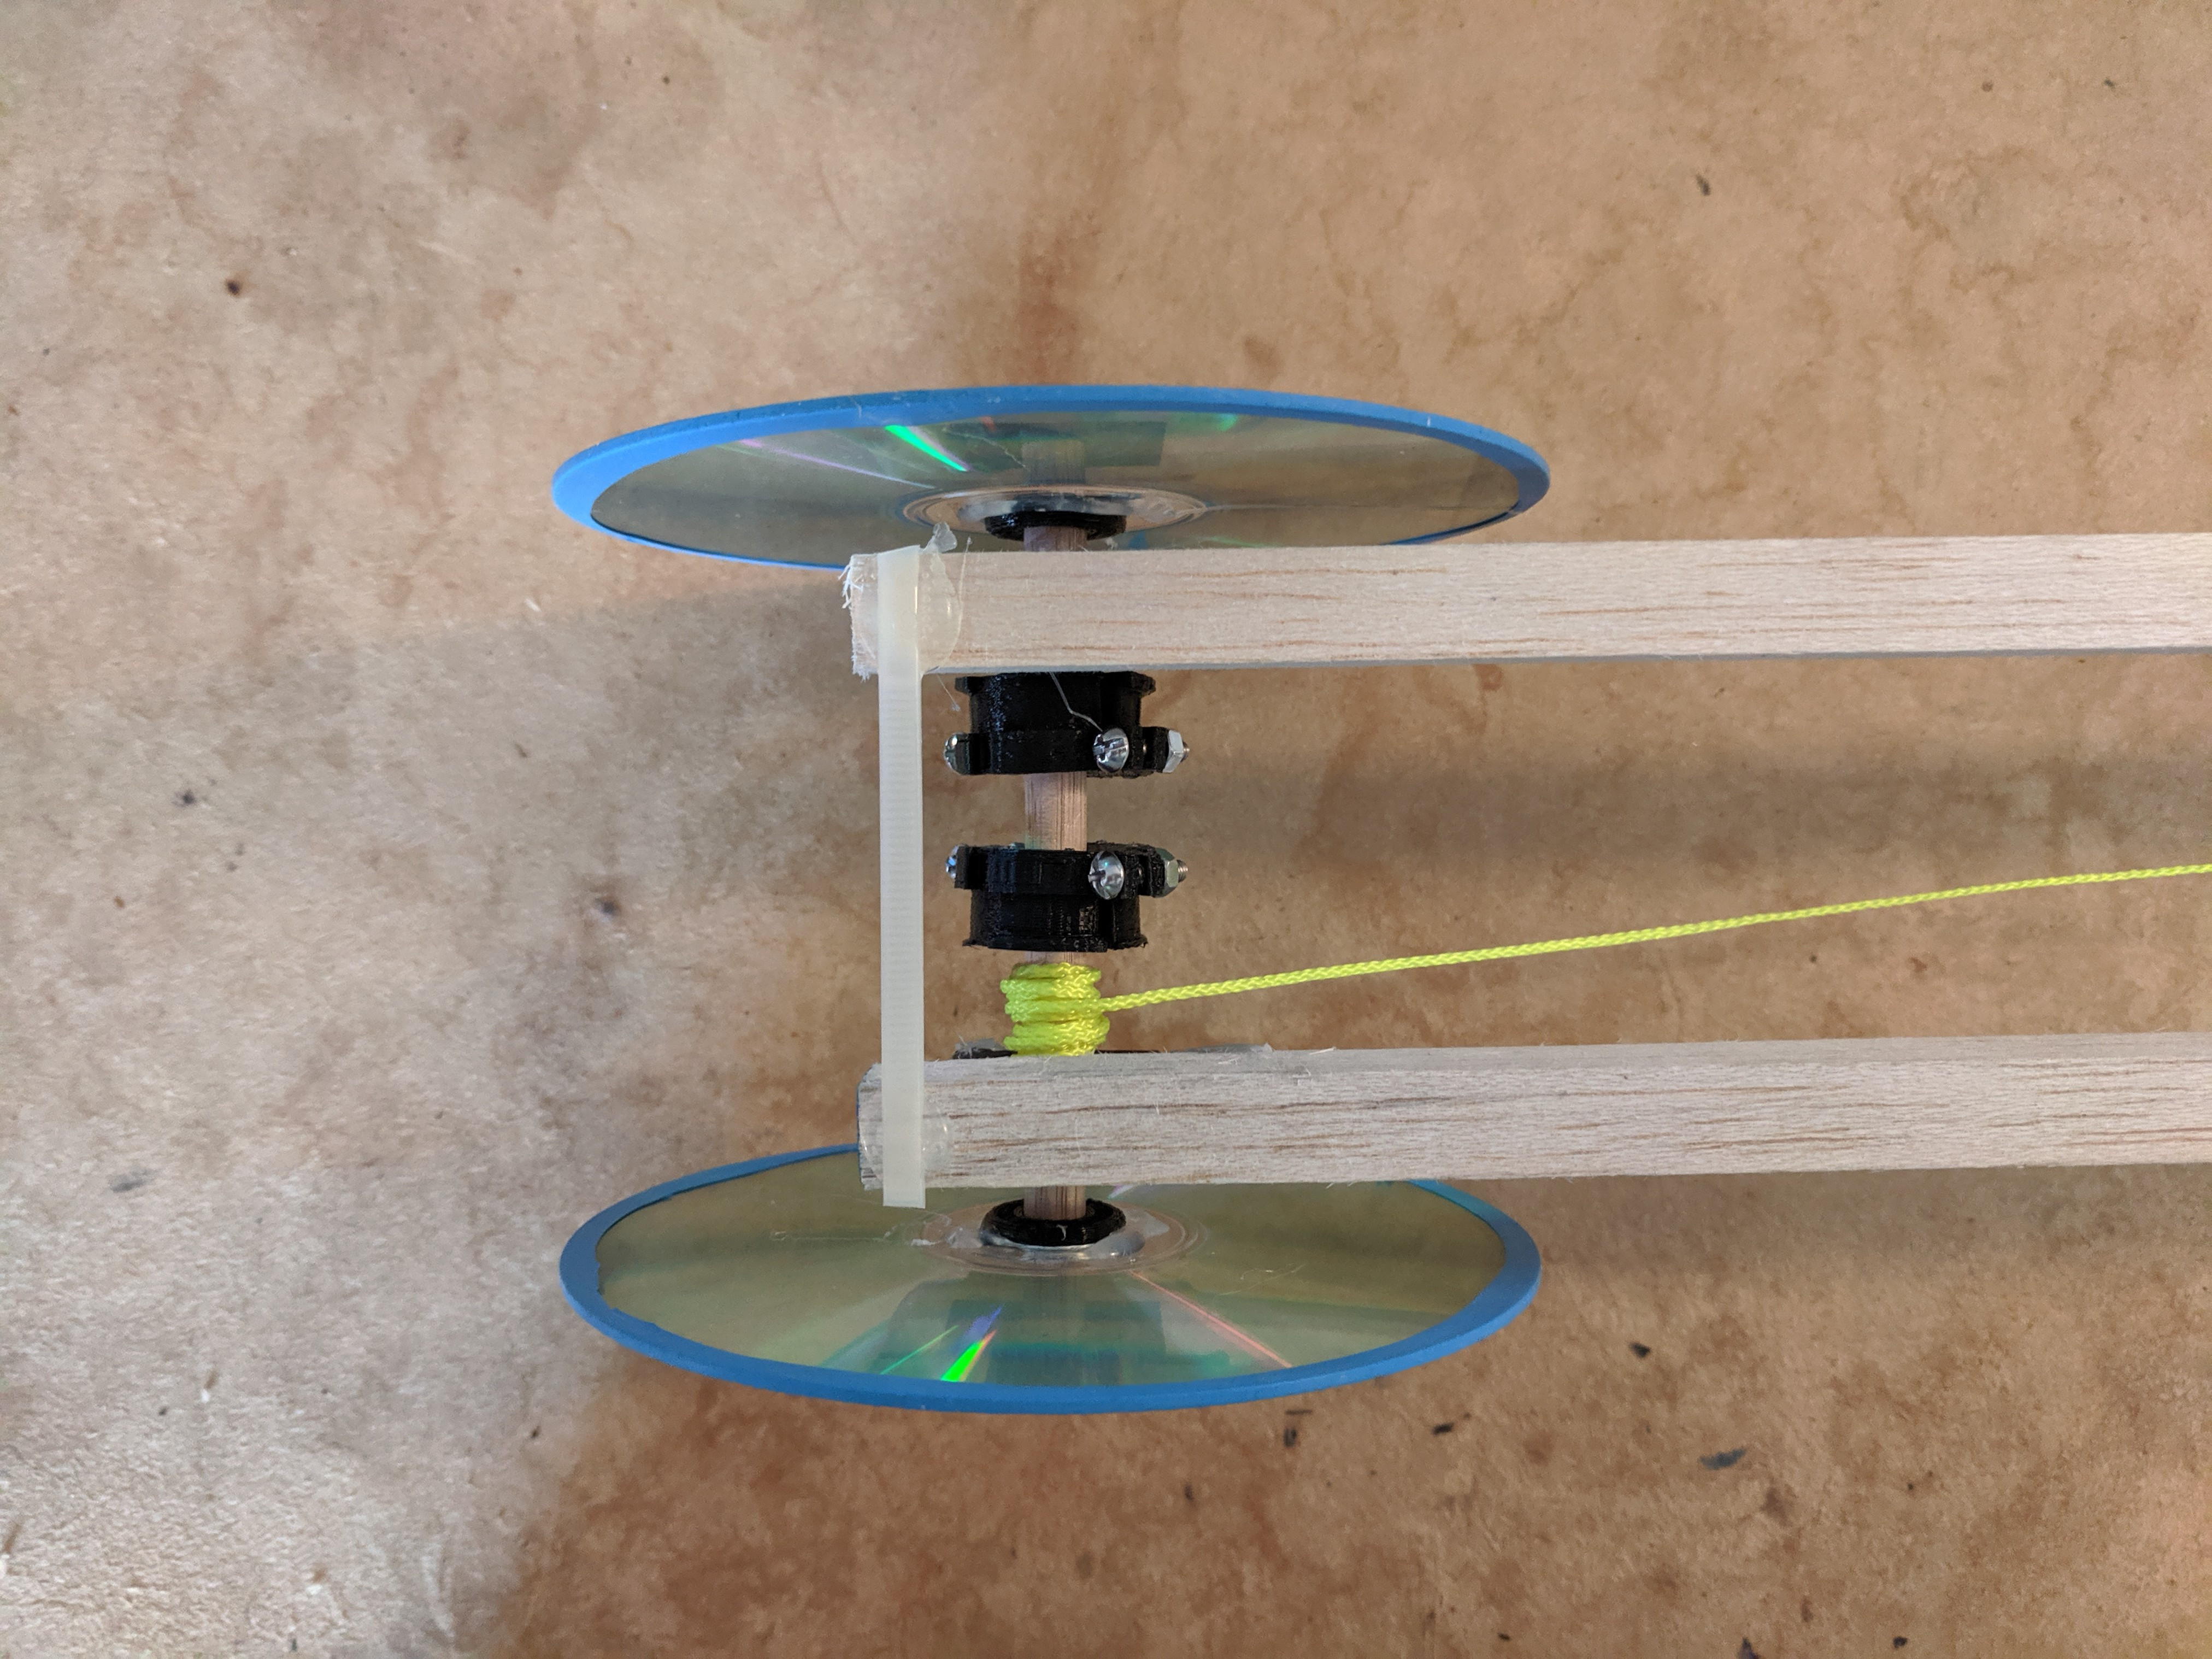
\includegraphics[height=5cm]{drive_shaft}}
		\caption{The string is wound around the drive shaft of the vehicle. When the string is tensioned the drive shaft experience torque and subsequent angular acceleration.}
	\end{minipage}
	\hspace{1cm}
	\begin{minipage}[t]{0.45\textwidth}
		\centering
		\frame{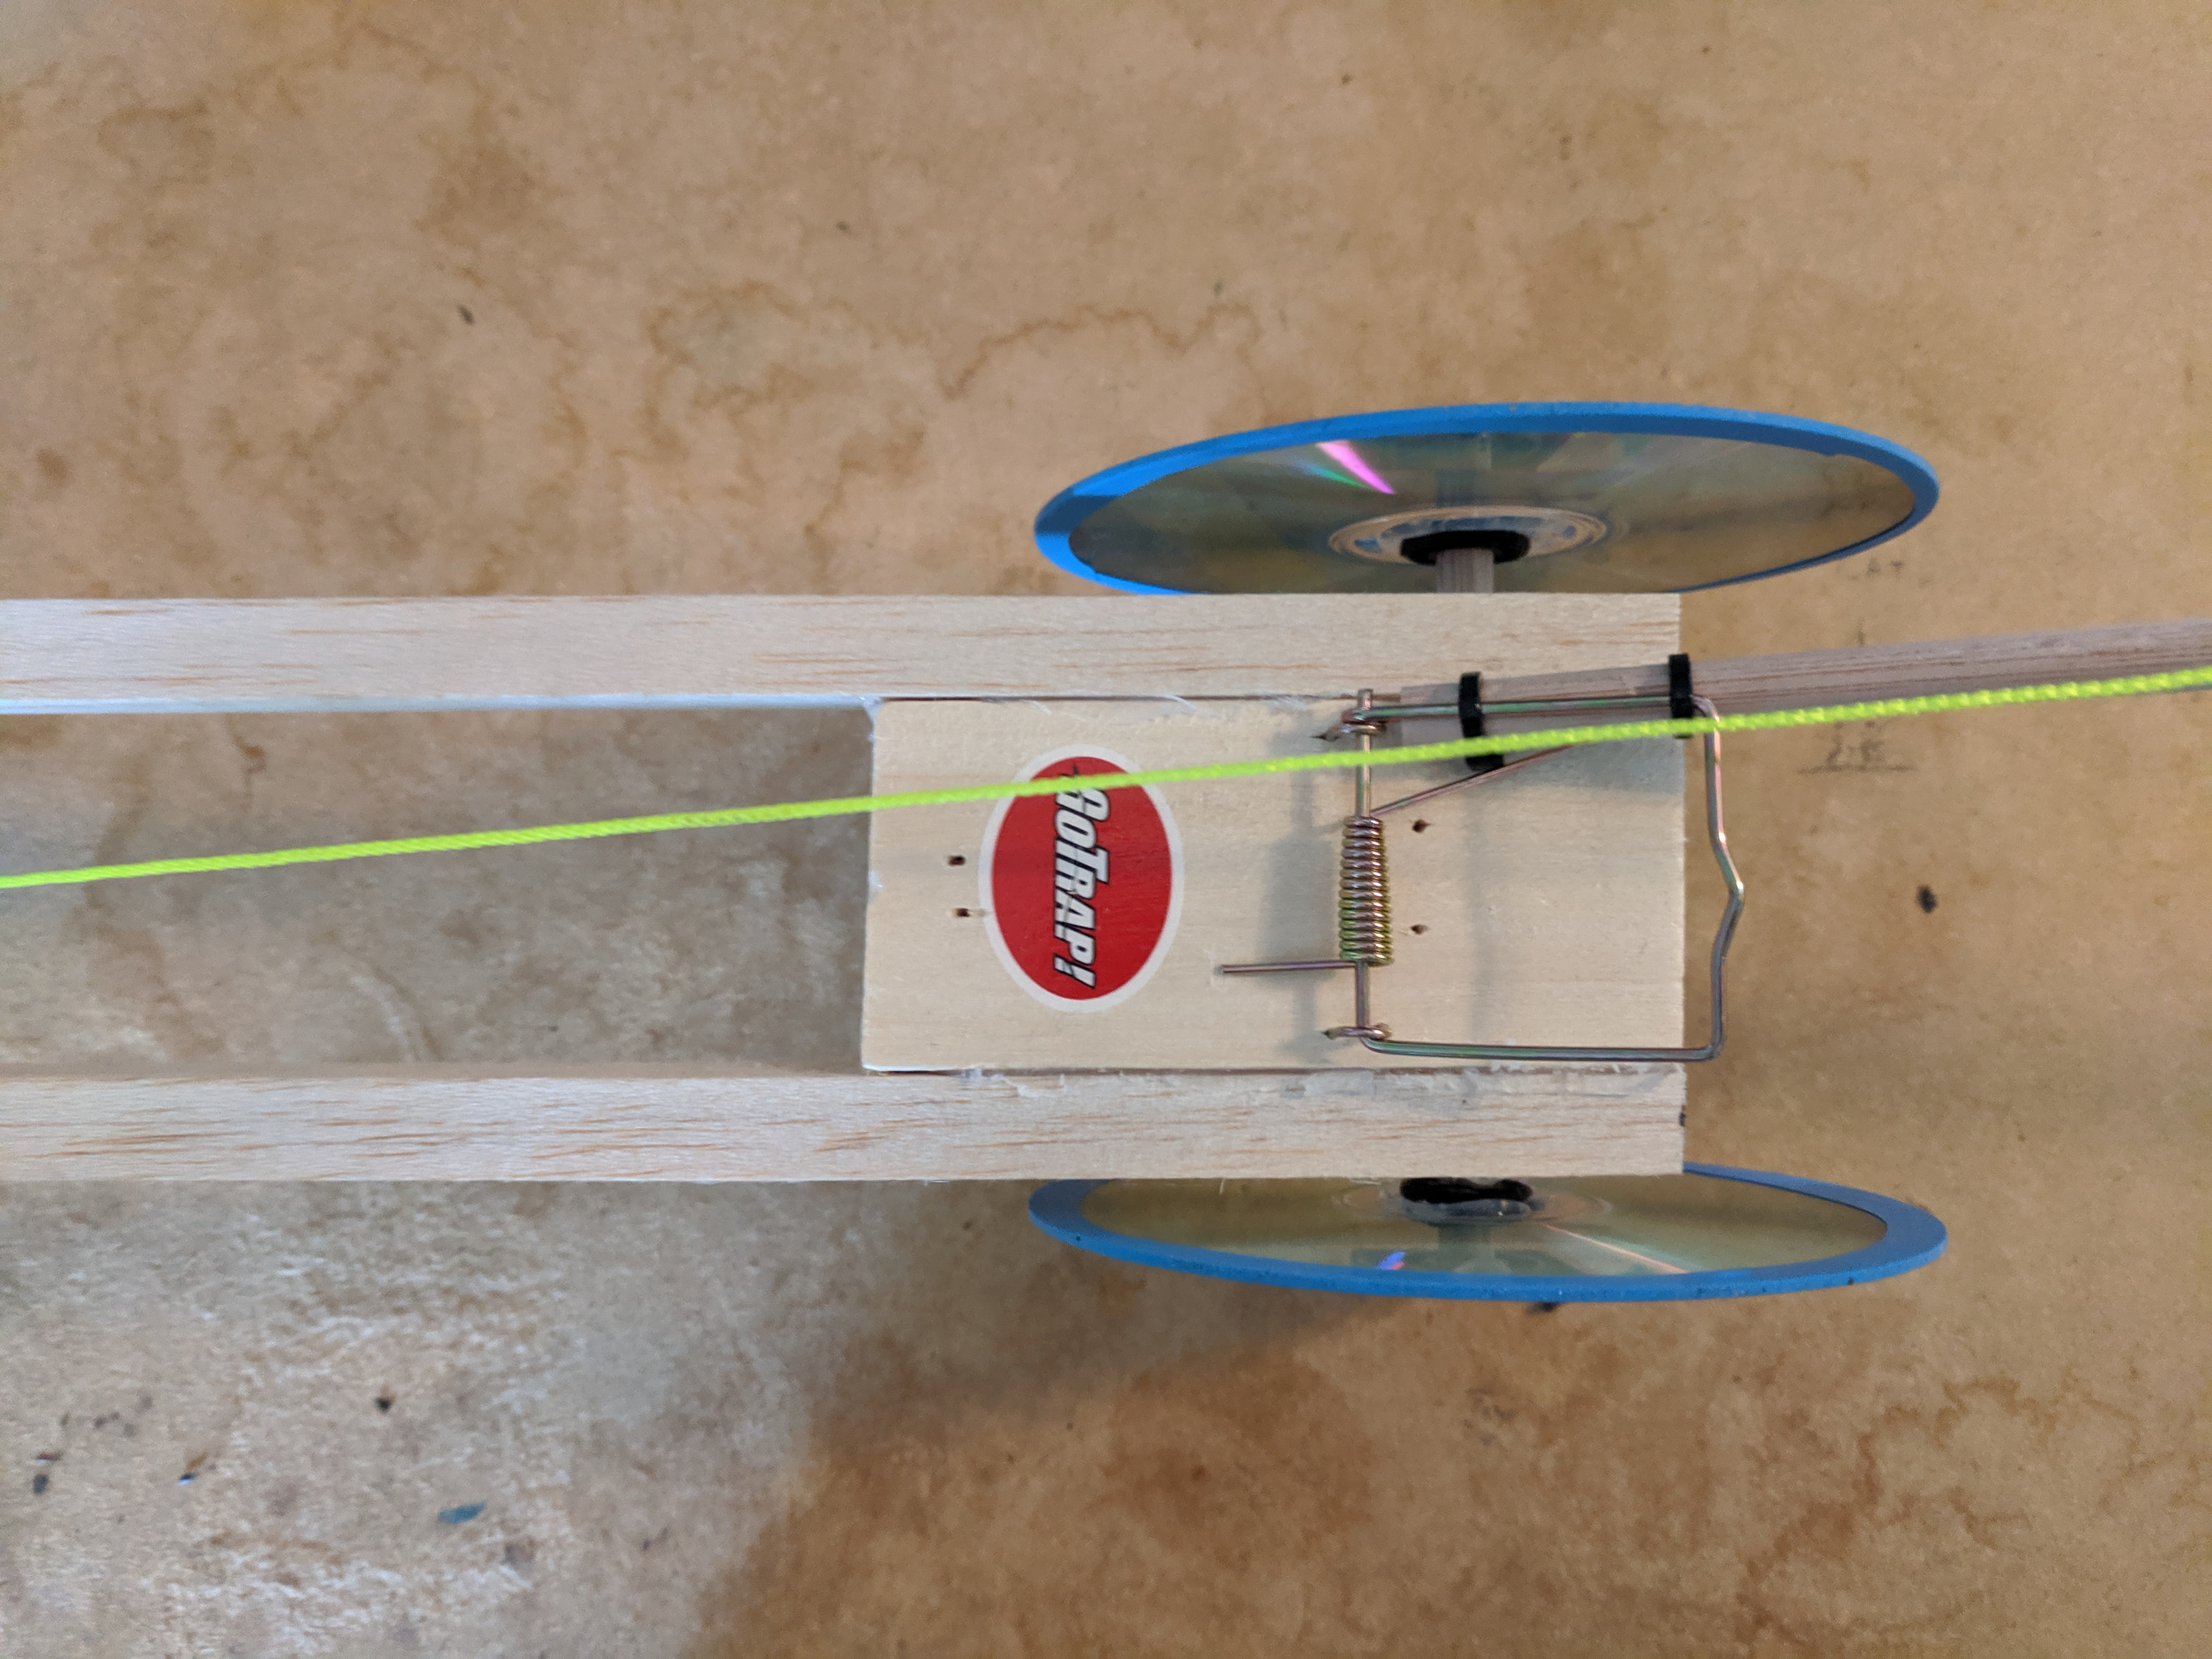
\includegraphics[height=5cm]{mouse_trap_lever}}
		\caption{The mouse trap has the dowel lever arm fixed to the side of the mouse trap.}
	\end{minipage}
\end{figure}

\begin{figure}[h]
	\centering
	\begin{minipage}[t]{0.45\textwidth}
		\centering
		\frame{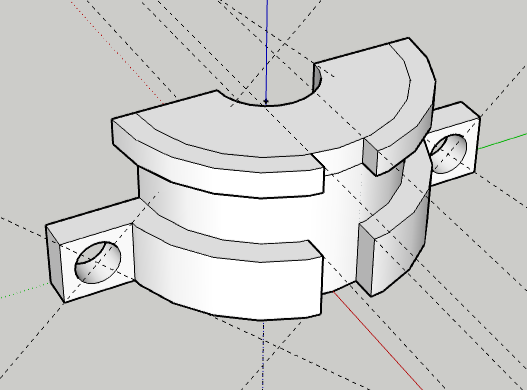
\includegraphics[height=5cm]{buffer}}
		\caption{A 3D model of a drive shaft buffer section created using Sketchp.}
	\end{minipage}
	\hspace{1cm}
	\begin{minipage}[t]{0.45\textwidth}
		\centering
		\frame{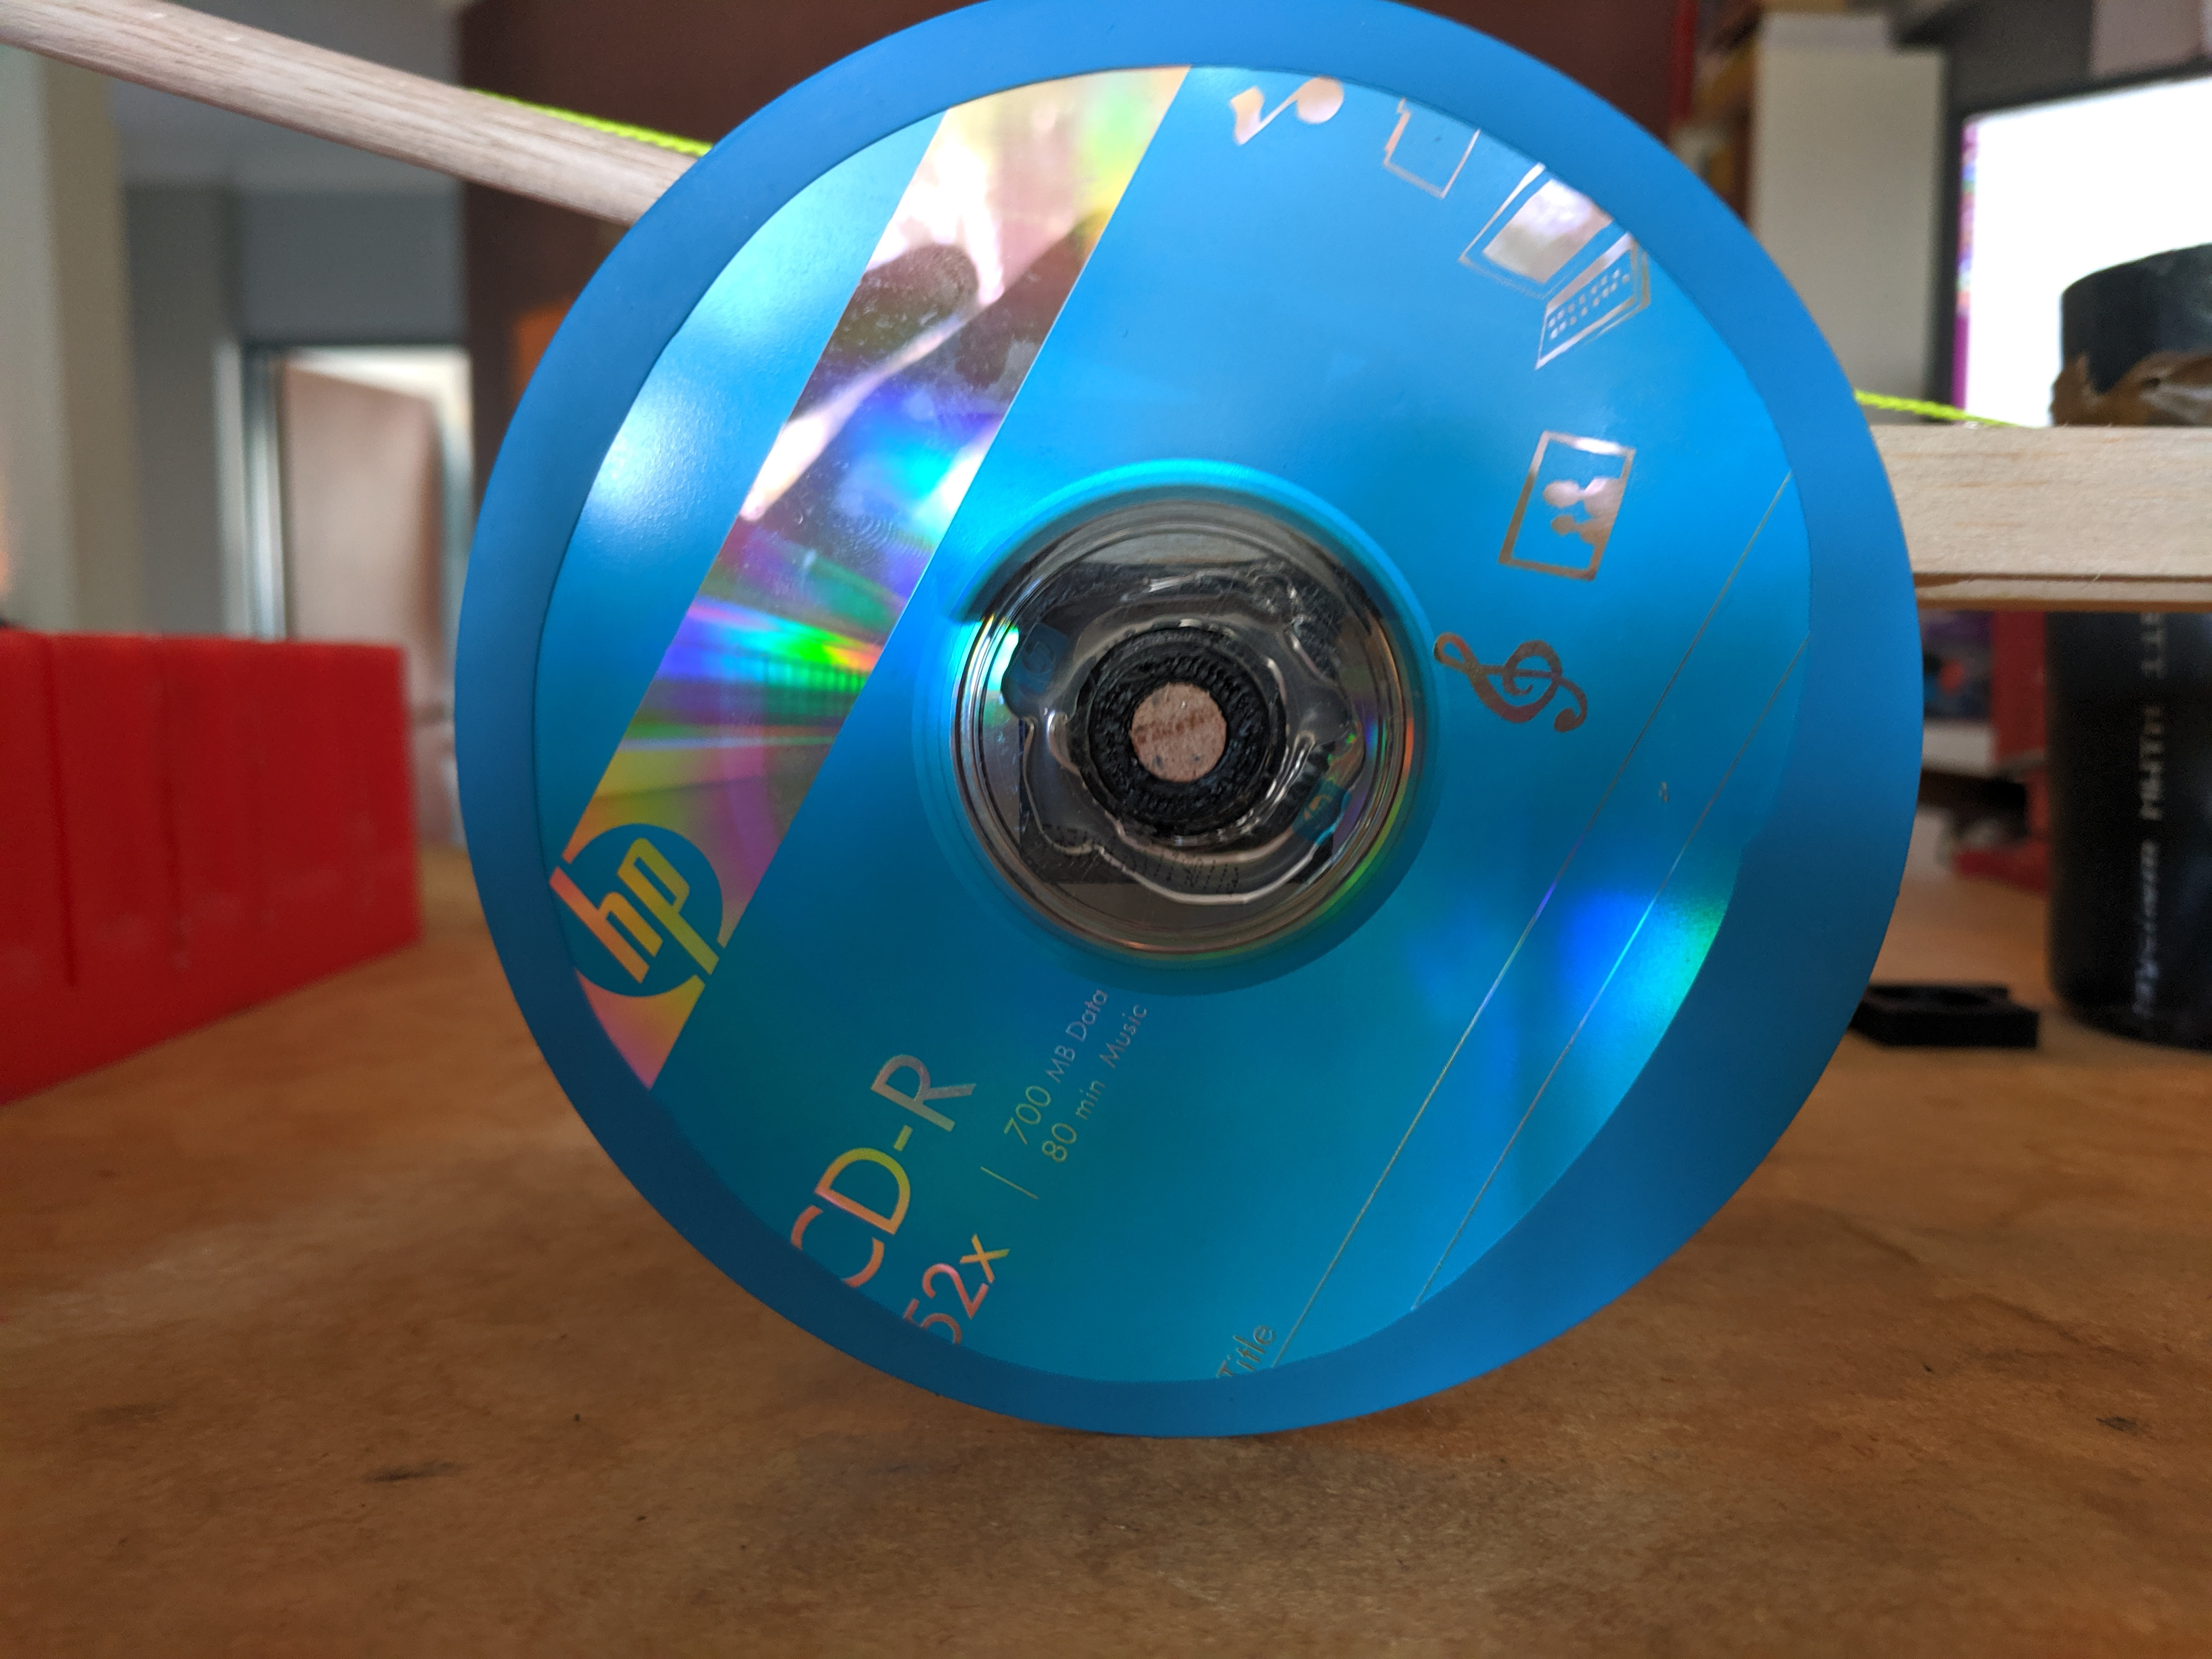
\includegraphics[height=5cm]{cd_wheel}}
		\caption{Wheels were carefully mounted to the shaft ensuring that the wheel centre of mass aligned with the axis of rotation, achieved using 3D printed mounts.}
	\end{minipage}
\end{figure}

Despite mass increases from the addition of buffers, the net result is a quicker round trip time. Drive shaft buffers were designed to be removed from shaft to allow for easy experimentation. A 3D model of a buffer section, created in SketchUp, can be seen in Figure 4. A further alteration was the inclusion of bearings to reduce friction on the drive shaft as it rotates. The net effect of this is to reduce the rolling friction of the vehicle, allowing less of the torsional spring potential energy to be lost to work against the rolling friction force. Information on the bearings can be found in Figure 9.

Material choice for vehicle design was informed by rapid prototyping using aluminium L sections, timber, and balsa wood for the vehicle chassis.

\begin{figure}[h]
	\centering
	\begin{minipage}[t]{0.45\textwidth}
		\centering
		\frame{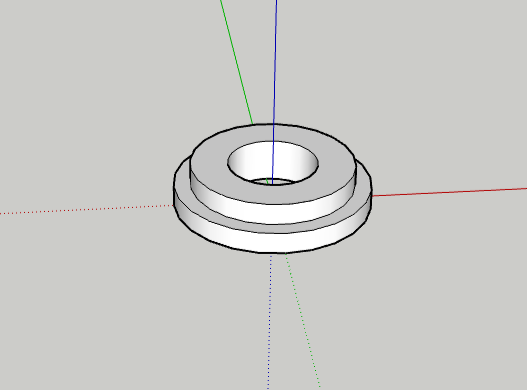
\includegraphics[height=5cm]{cd_mount_design}}
		\caption{Small plastic mounts designed to securely fix the shaft to the Compact Disc wheel at the centre of mass.}
	\end{minipage}
	\hspace{1cm}
	\begin{minipage}[t]{0.45\textwidth}
		\centering
		\frame{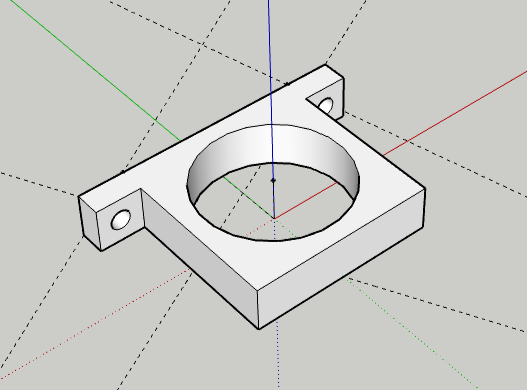
\includegraphics[height=5cm]{bearing_mount_design}}
		\caption{Small plastic mounts designed to house the bearings and attach them securely to the vehicle chassis.}
	\end{minipage}
\end{figure}

\begin{figure}[h]
	\centering
	\begin{minipage}[t]{0.45\textwidth}
		\centering
		\begin{tabular}{p{3.5cm}rc}
			\toprule
			Measurement & Value & Unit \\
			\midrule
			Length & 0.450 & $\si{\meter}$ \\
			Width & 0.010 & $\si{\meter}$  \\
			Mass & 0.006 & $\si{\kilogram}$ \\
			\bottomrule
		\end{tabular}
		
		\vspace{0.5cm}
		
		\frame{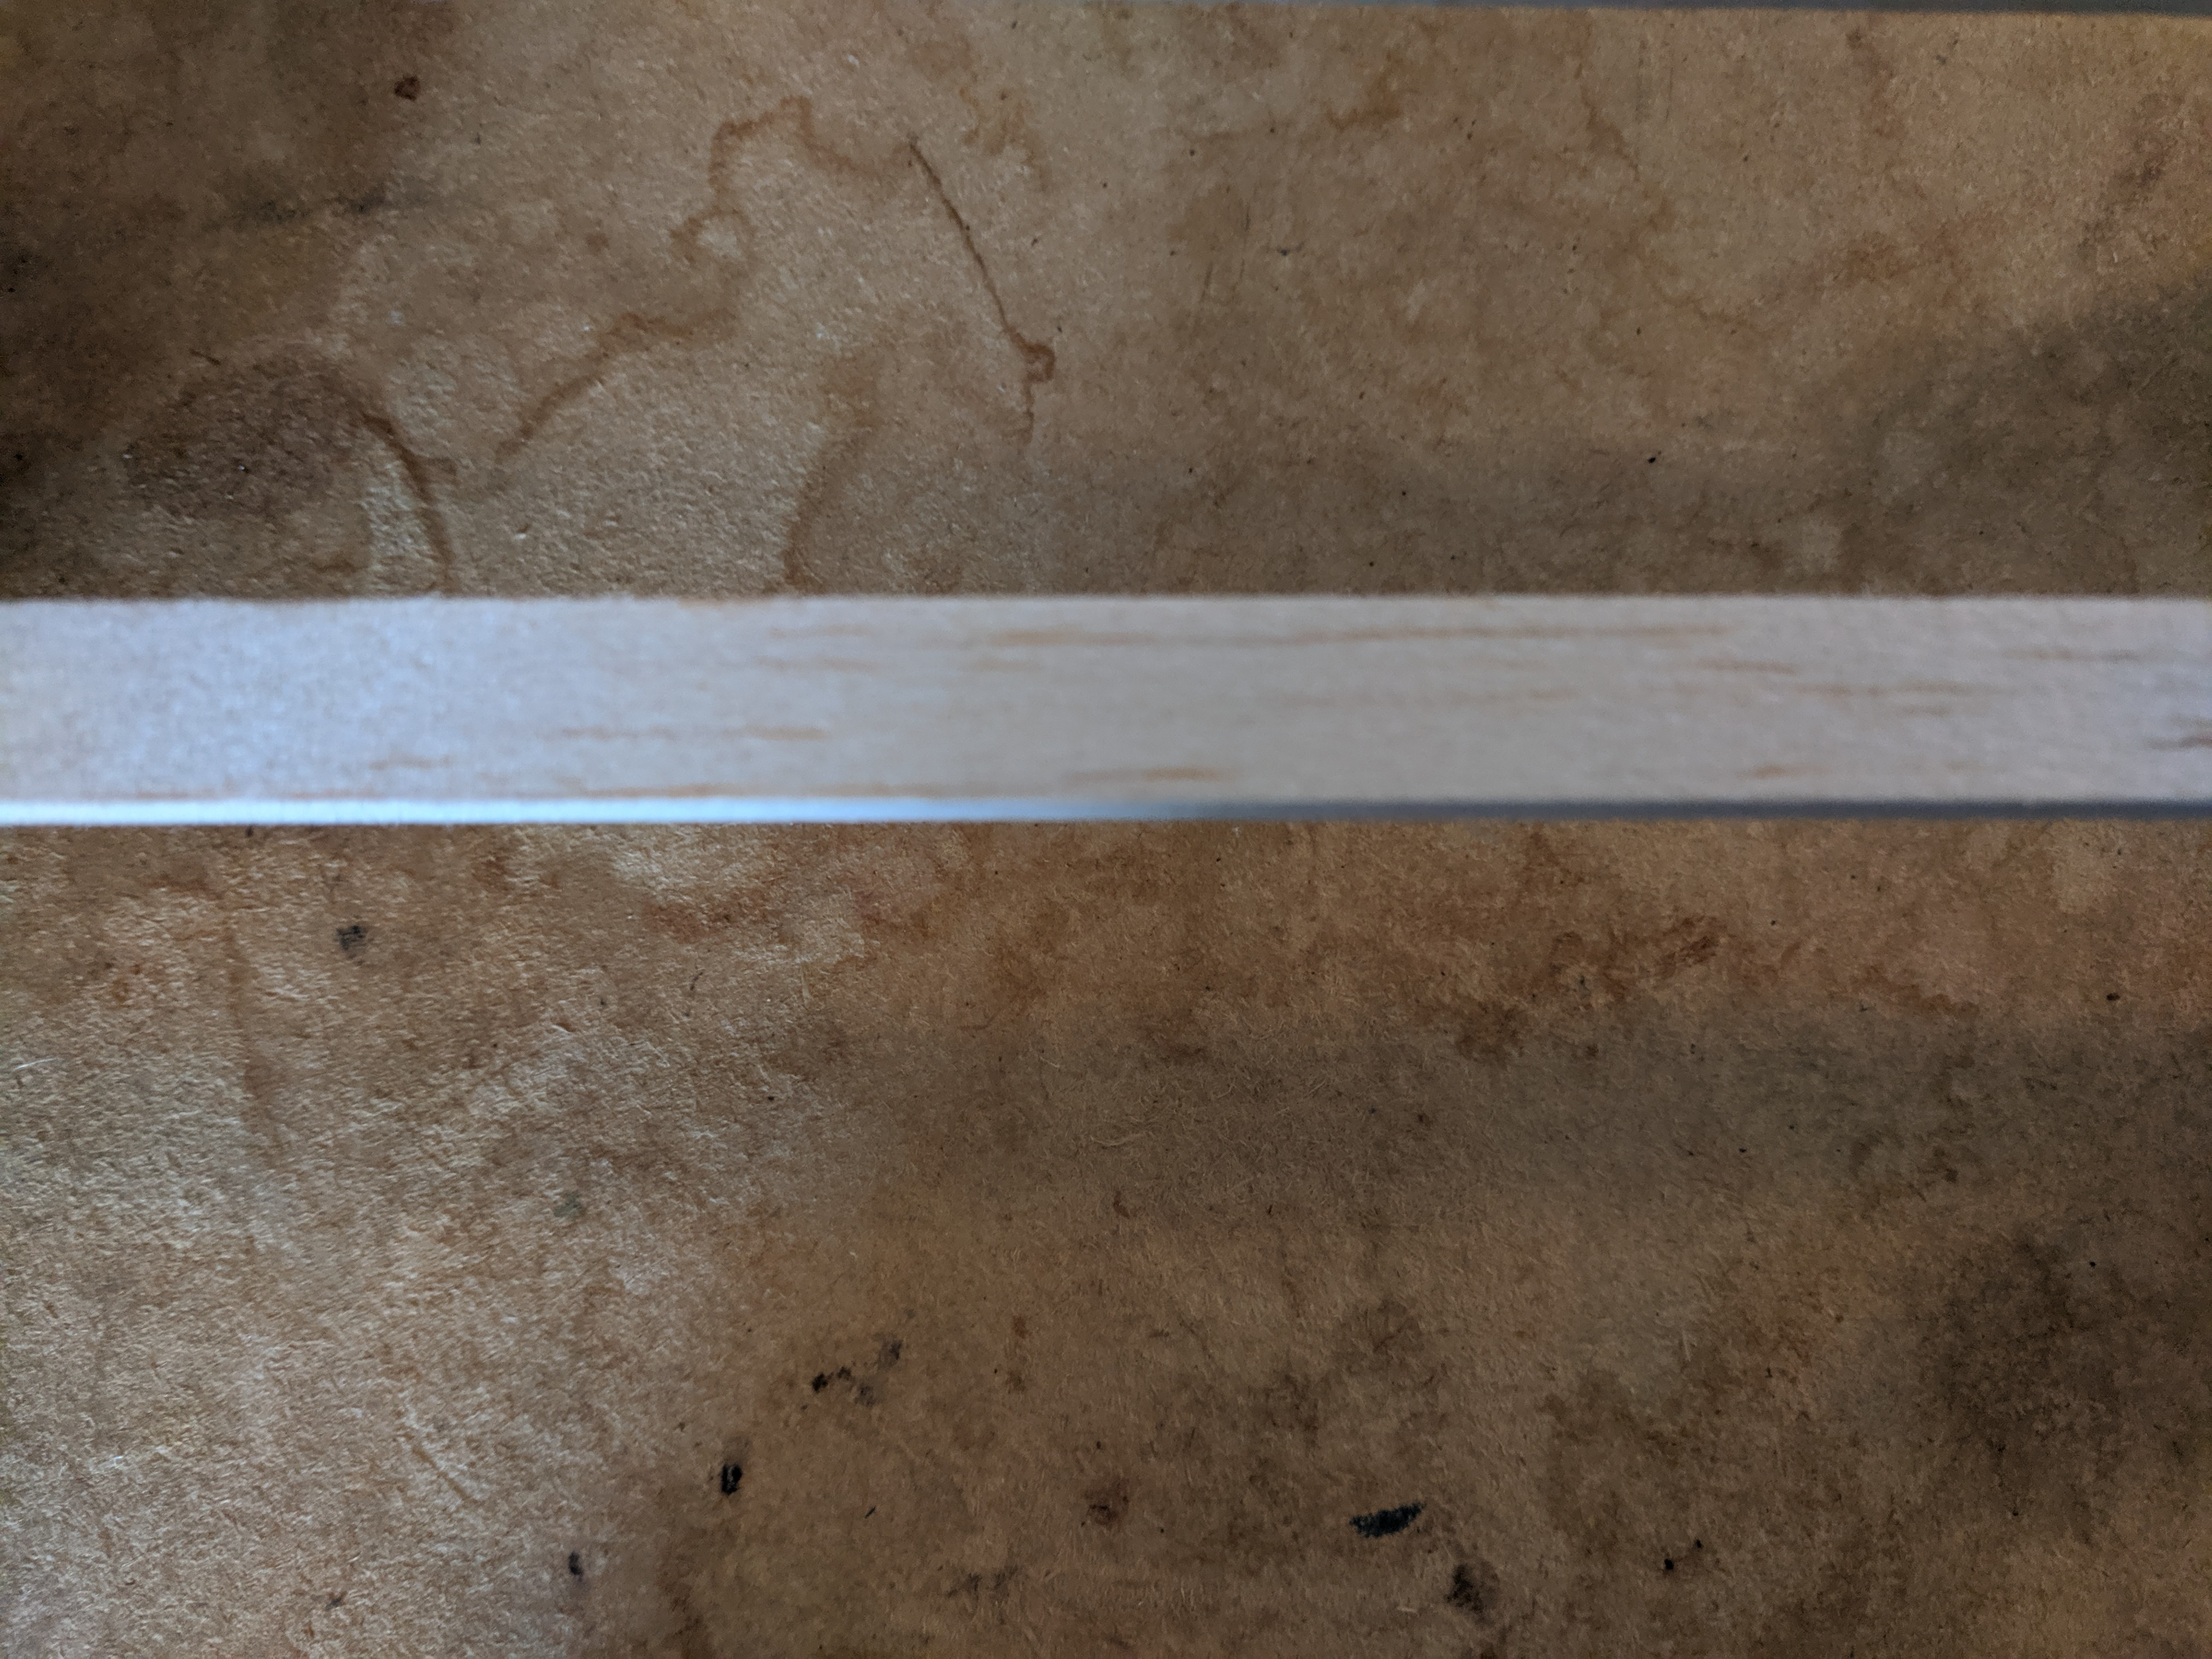
\includegraphics[height=5cm]{balsa_frame}}
		\caption{Balsa wood section used for the frame. Two lengths were used.}
	\end{minipage}
	\hspace{1cm}
	\begin{minipage}[t]{0.45\textwidth}
		\centering
		\begin{tabular}{p{3.5cm}rc}
			\toprule
			Measurement & Value & Unit \\
			\midrule
			Diameter & 0.022 & $\si{\meter}$ \\
			Mass & 0.009 & $\si{\kilogram}$ \\
			 & & \\
			\bottomrule
		\end{tabular}
		
		\vspace{0.5cm}
		
		\frame{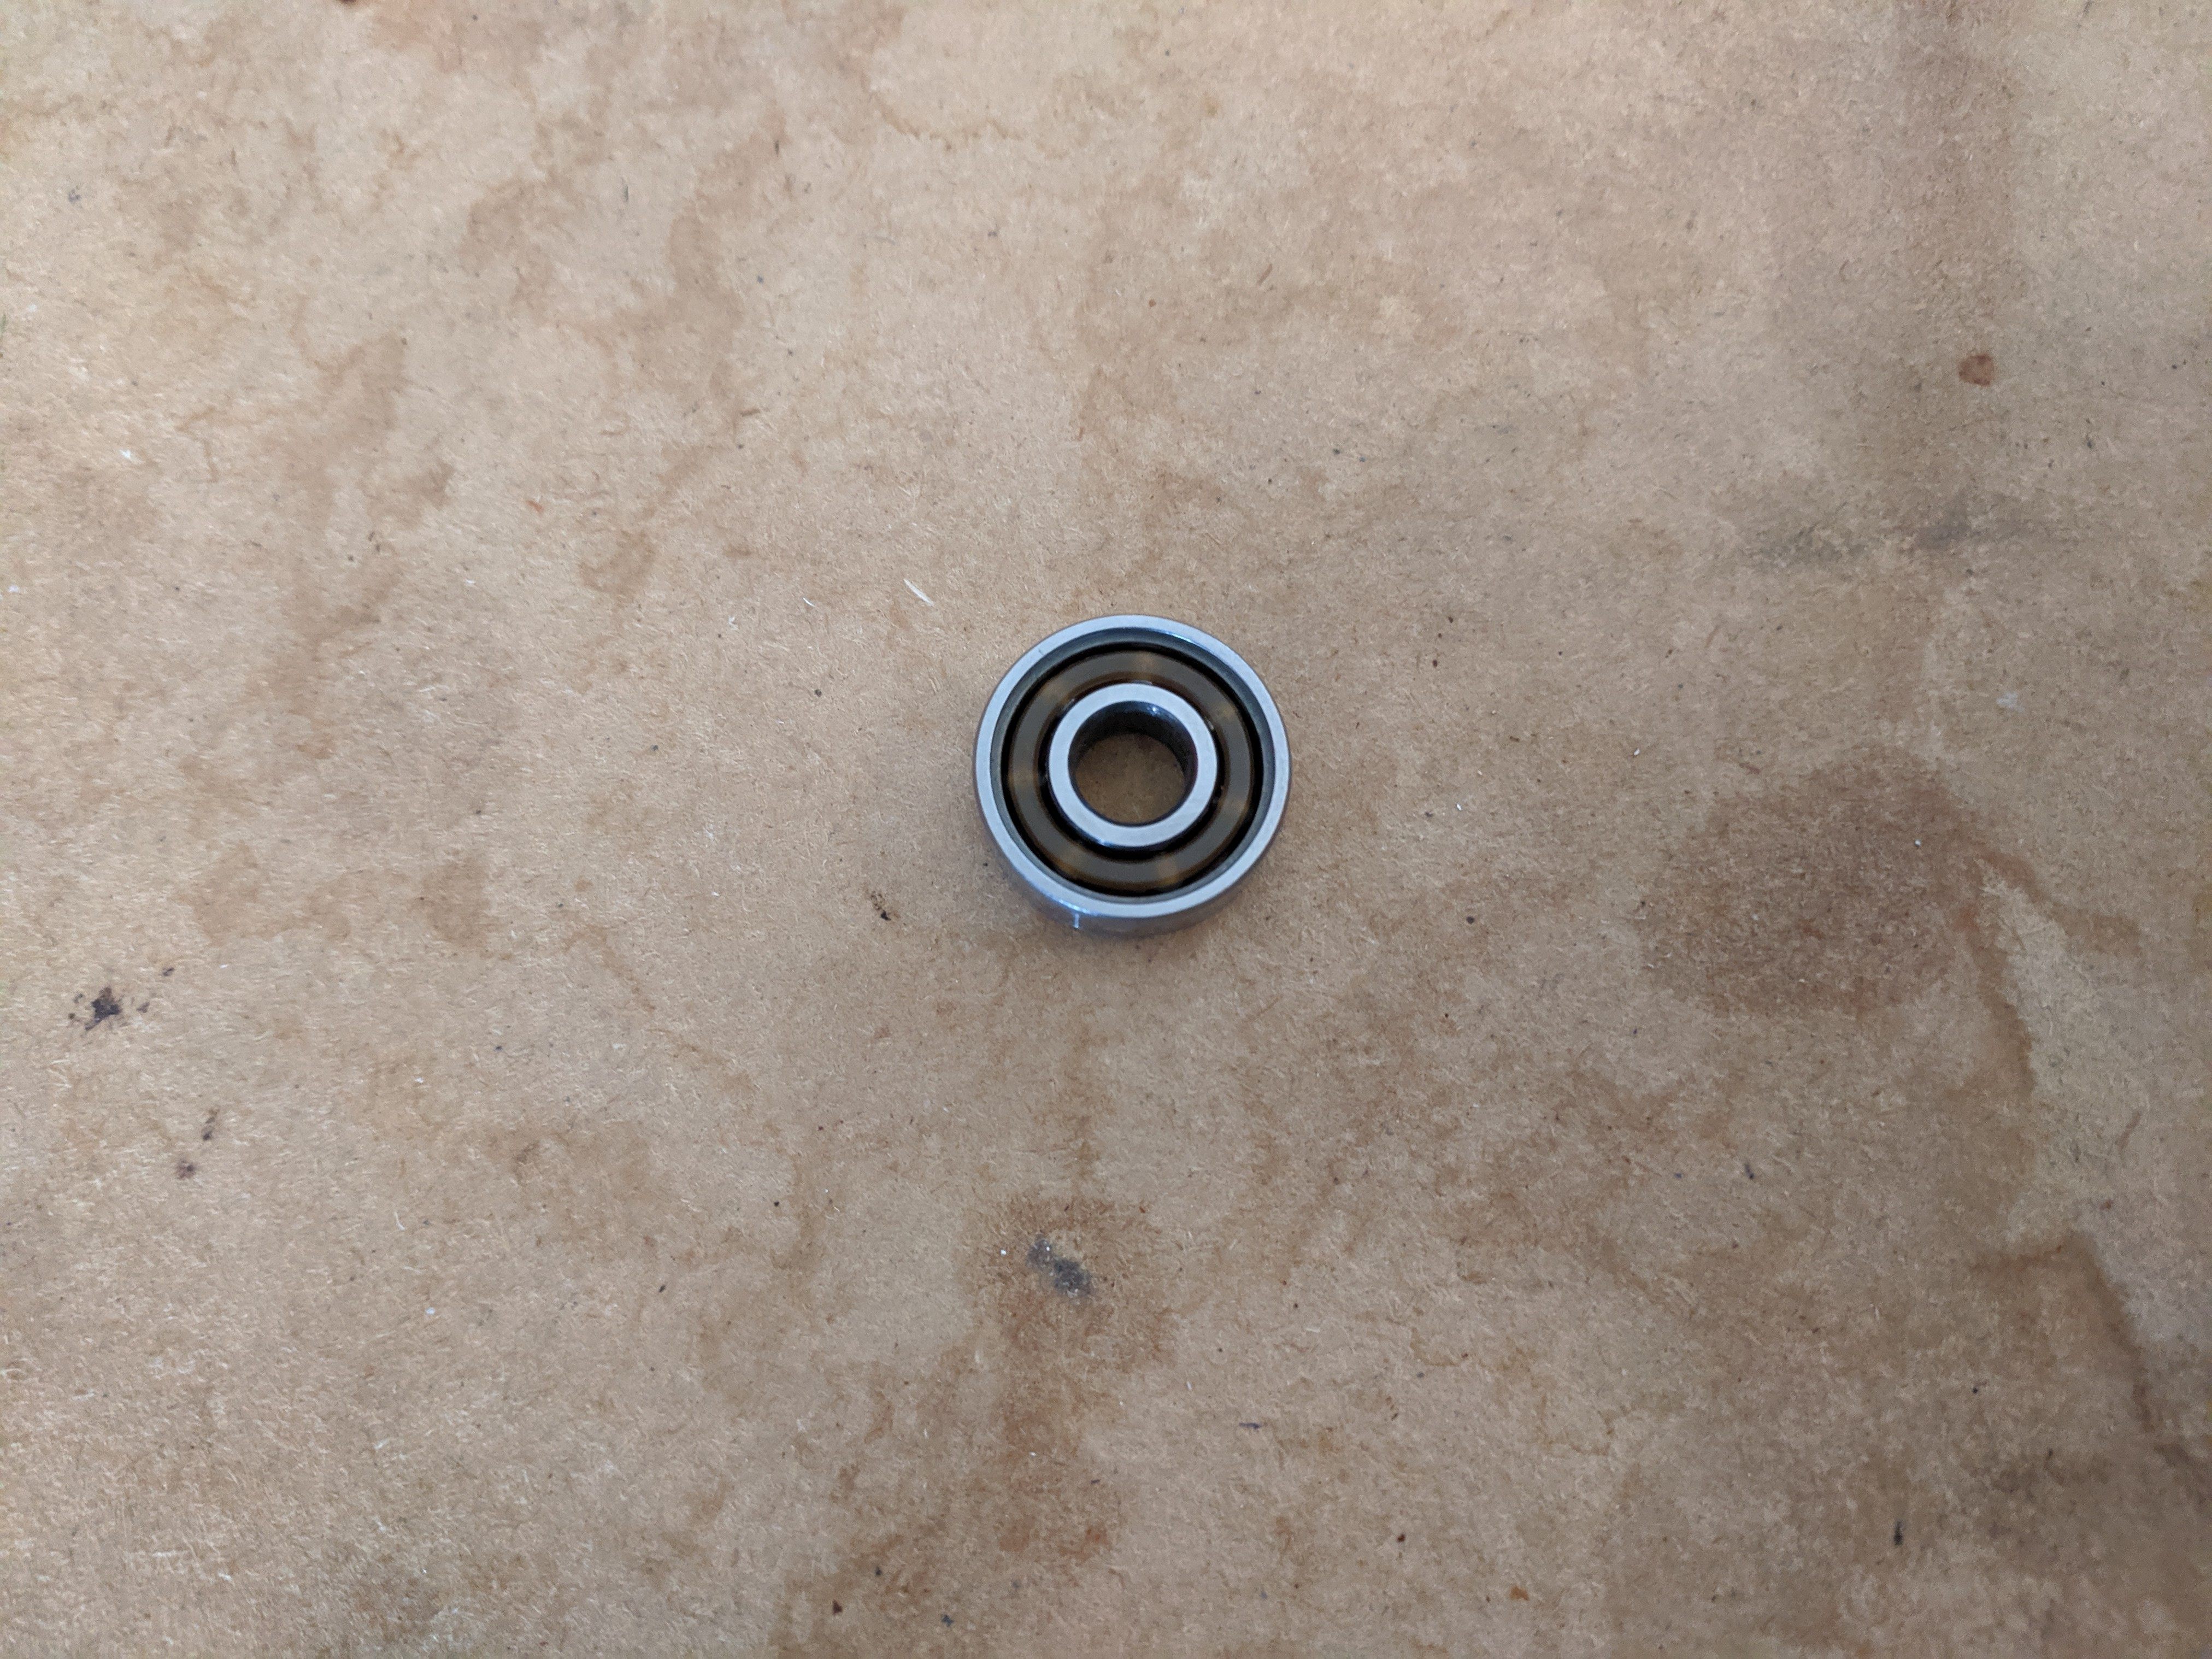
\includegraphics[height=5cm]{bearing}}
		\caption{Bearings used to reduce friction between shafts and frame.}
	\end{minipage}
\end{figure}


\begin{figure}[h]
	\centering
	\begin{minipage}[t]{0.45\textwidth}
		\centering
		
		\begin{tabular}{p{3.5cm}rc}
			\toprule
			Measurement & Value & Unit \\
			\midrule
			Length & 0.028 & $\si{\meter}$ \\
			Width & 0.028 & $\si{\meter}$ \\
			Mass & 0.002 & $\si{\kilogram}$ \\
			\bottomrule
		\end{tabular}
		
		\vspace{0.5cm}
		
		\frame{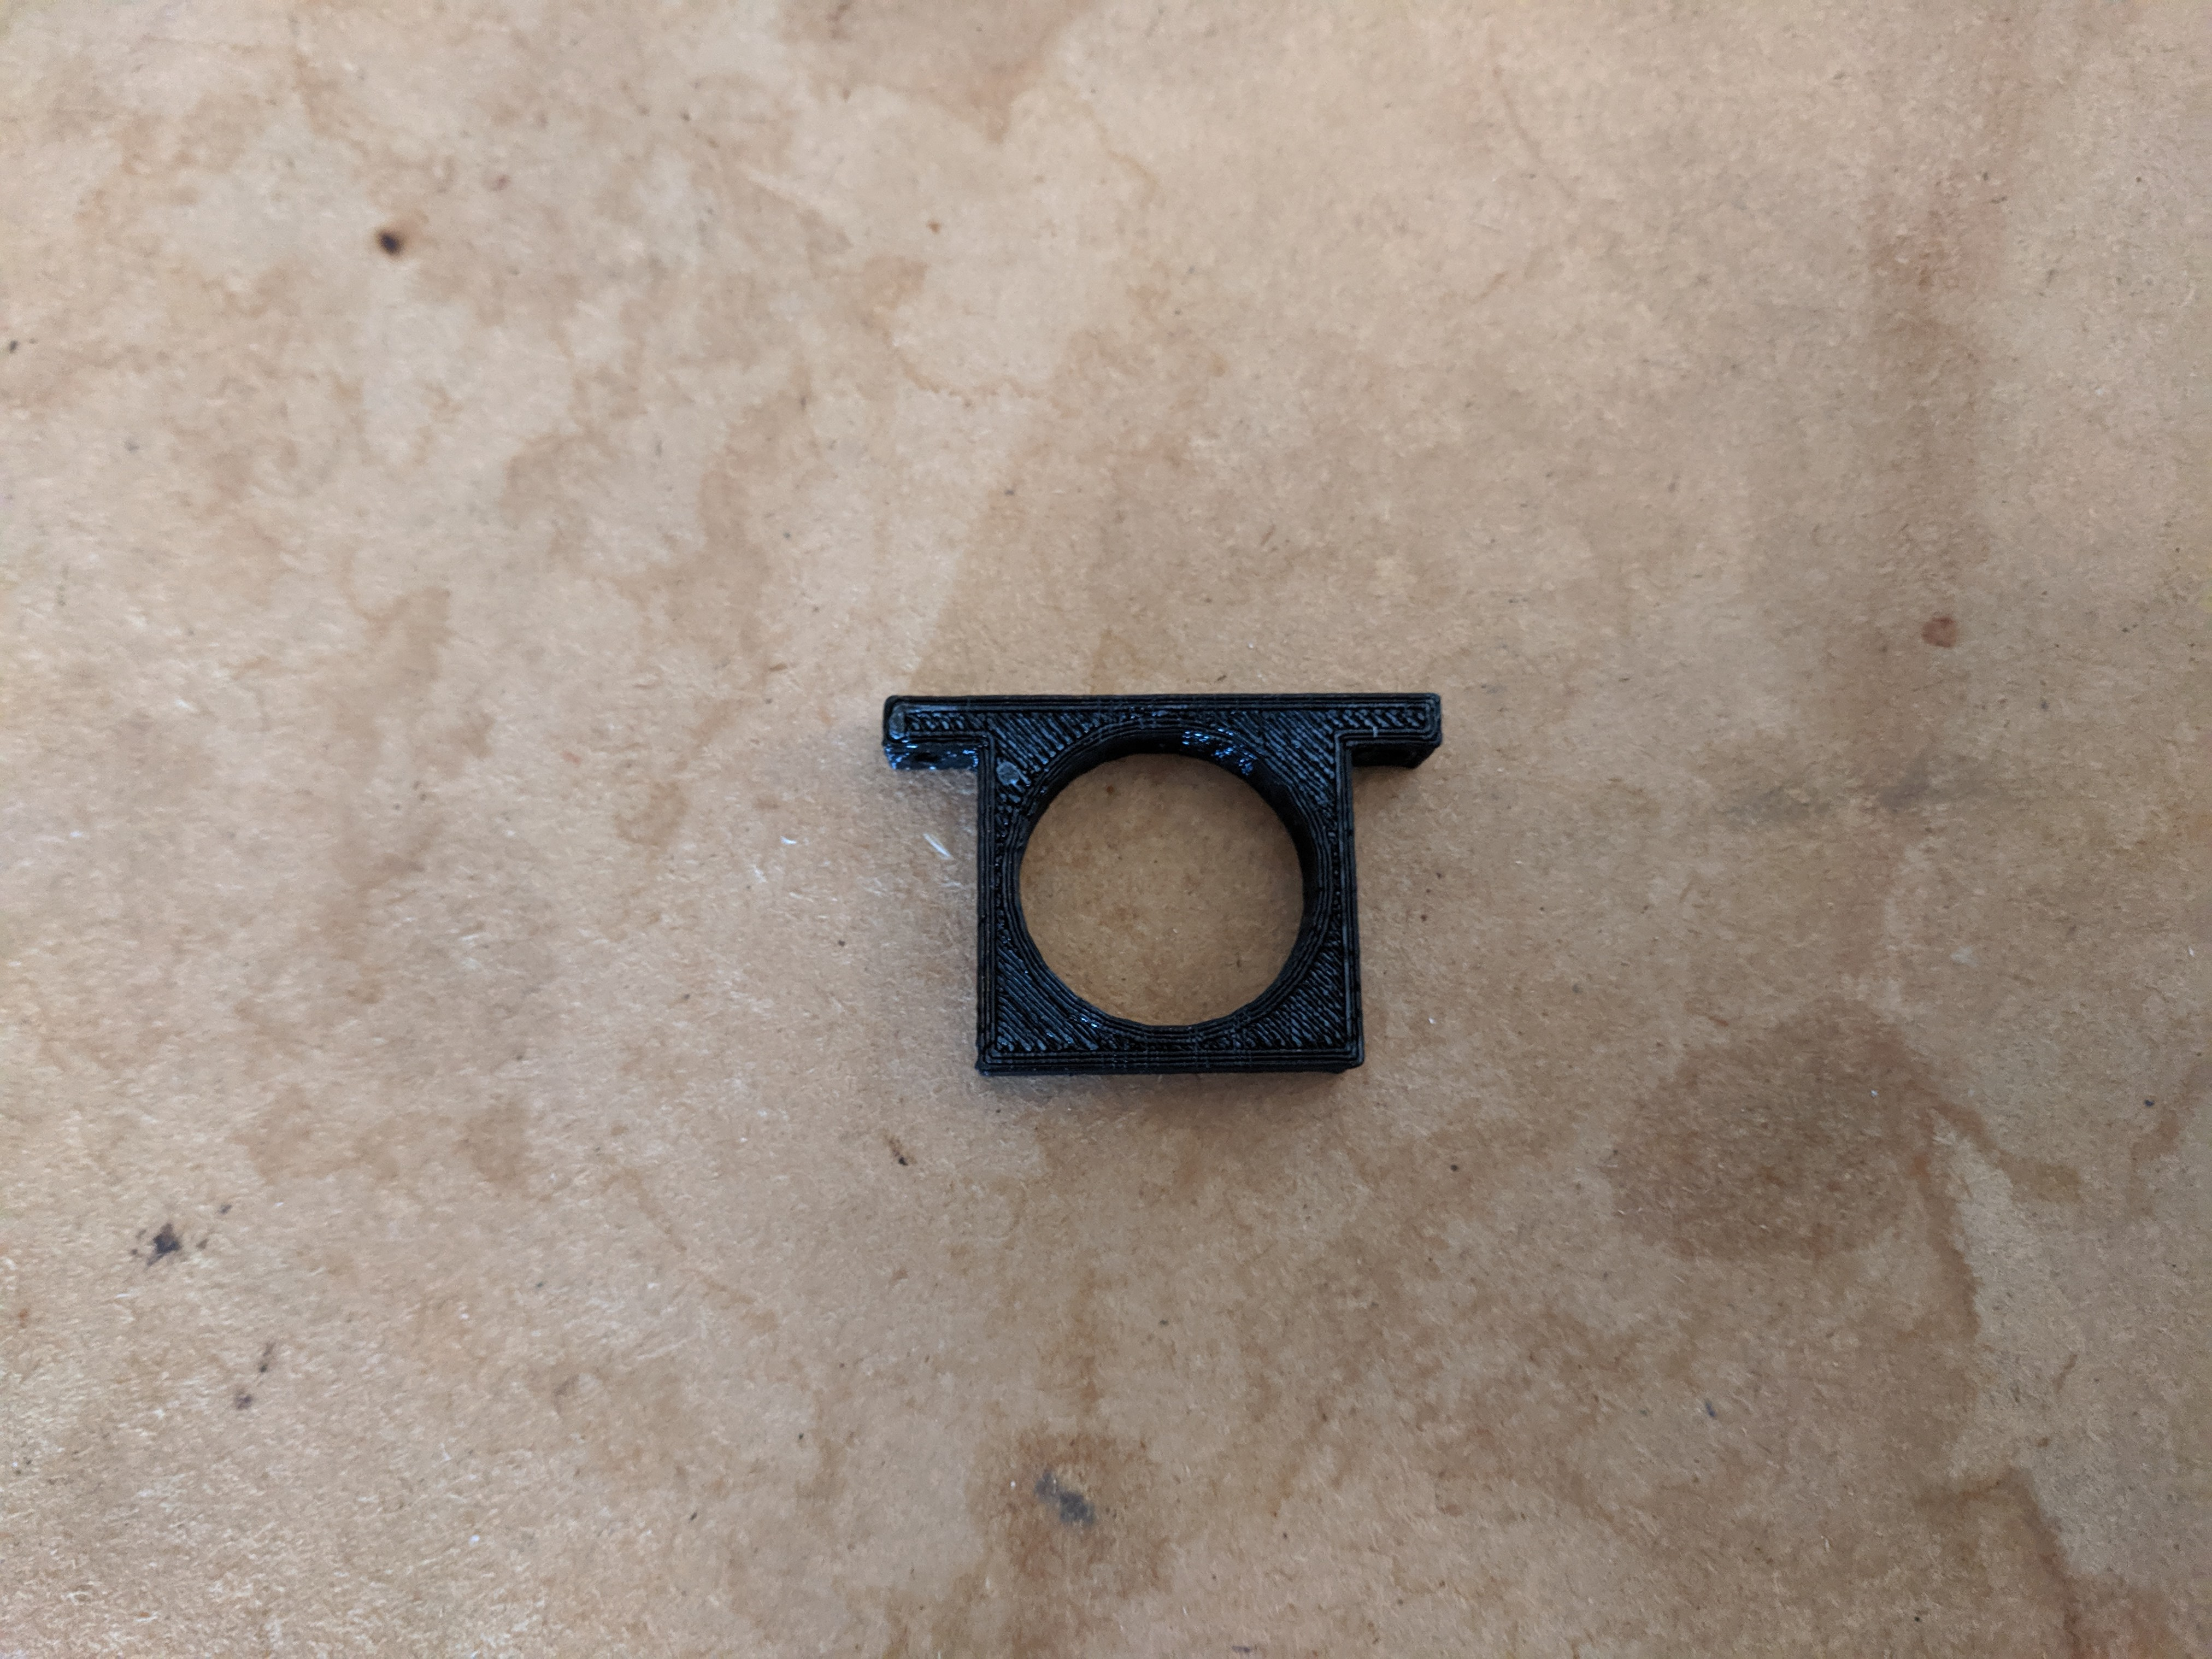
\includegraphics[height=5cm]{bearing_mount}}
		\caption{Plastic bearing mounts designed with Sketch up and constructed using additive manufacturing. Four of these were used.}
	\end{minipage}
	\hspace{1cm}
	\begin{minipage}[t]{0.45\textwidth}
		\centering
		
		\begin{tabular}{p{3.5cm}lr}
			\toprule
			Measurement & Value & Unit \\
			\midrule
			Diameter & 0.120 & $\si{\meter}$ \\
			Mass & 0.013 & $\si{\kilogram}$ \\
			 & & \\
			\bottomrule
		\end{tabular}
		
		\vspace{0.5cm}
		
		\frame{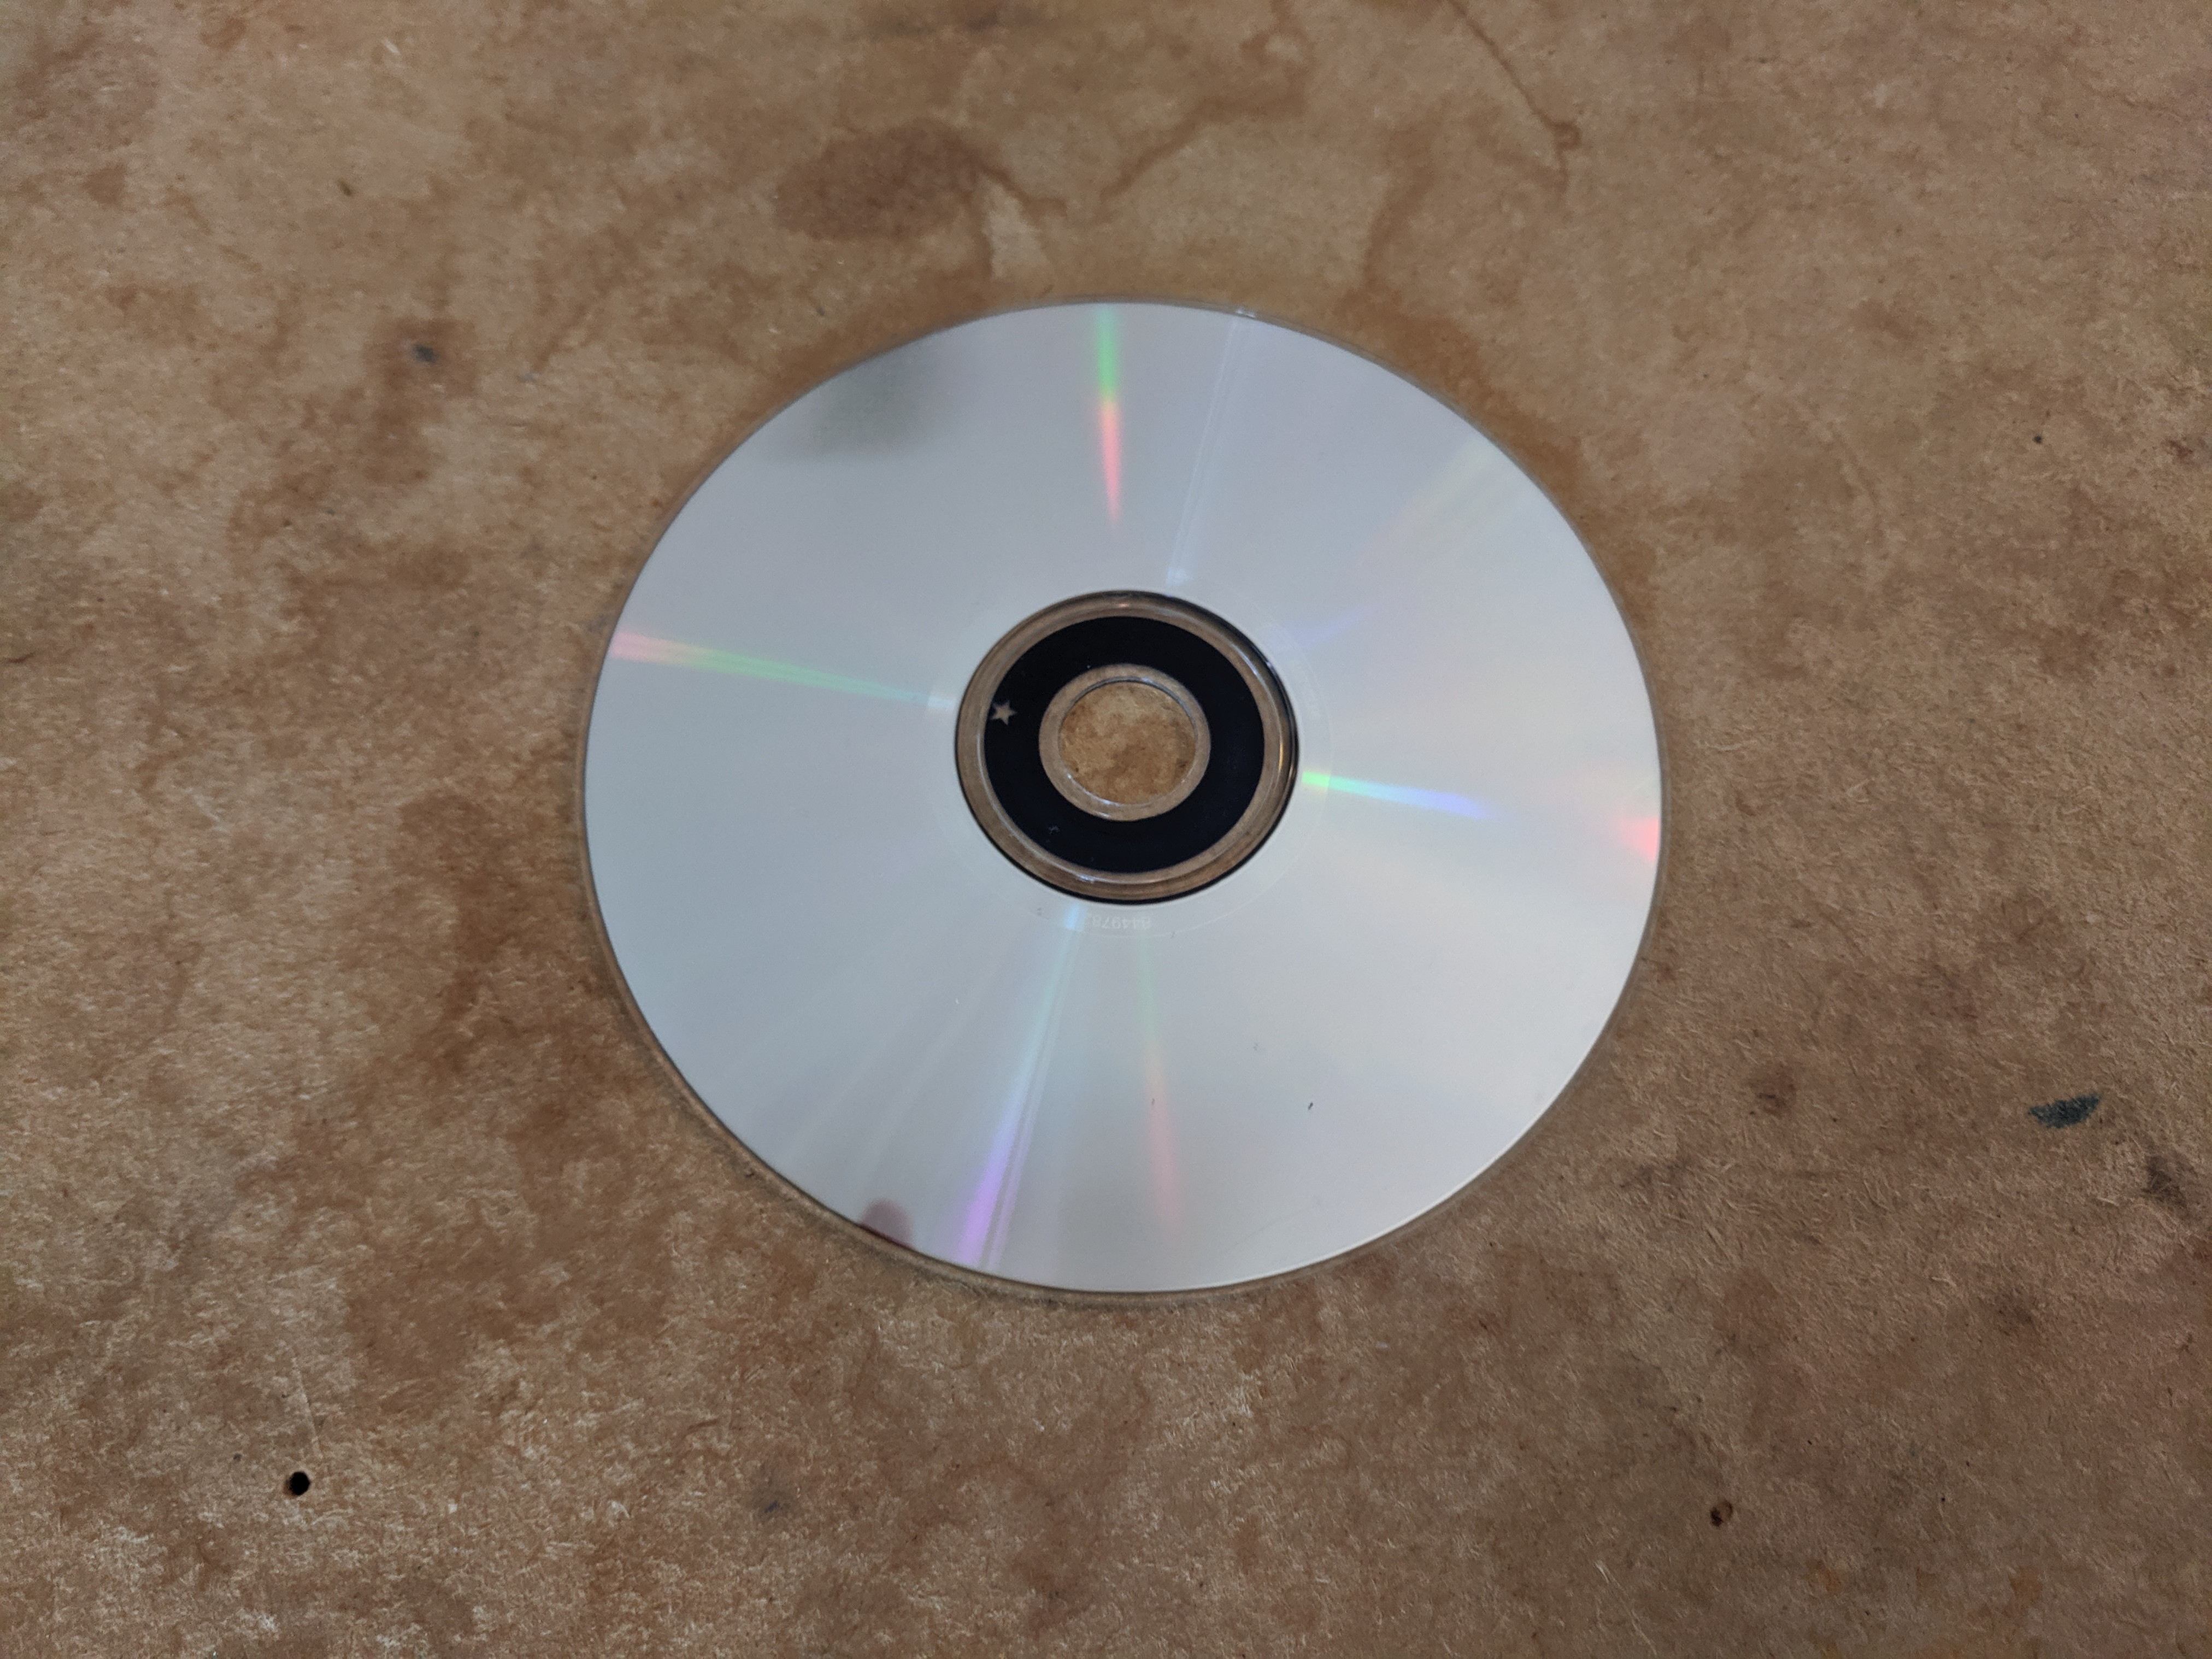
\includegraphics[height=5cm]{cd}}
		\caption{Compact disc used for wheels. Four of these were used.}
	\end{minipage}
\end{figure}


\begin{figure}[h]
	\centering
	\begin{minipage}[t]{0.45\textwidth}
		\centering
		\begin{tabular}{p{3.5cm}rc}
			\toprule
			Measurement & Value & Unit \\
			\midrule
			Length (Lever Arm) & 0.400 & $\si{\meter}$ \\
			Length (Shaft) & 0.100 & $\si{\meter}$ \\
			Mass (Lever Arm) & 0.011 & $\si{\si{\kilogram}}$ \\
			Mass (Lever Arm) & 0.003 & $\si{\si{\kilogram}}$ \\
			\bottomrule
		\end{tabular}
		
		\vspace{0.5cm}
		
		\frame{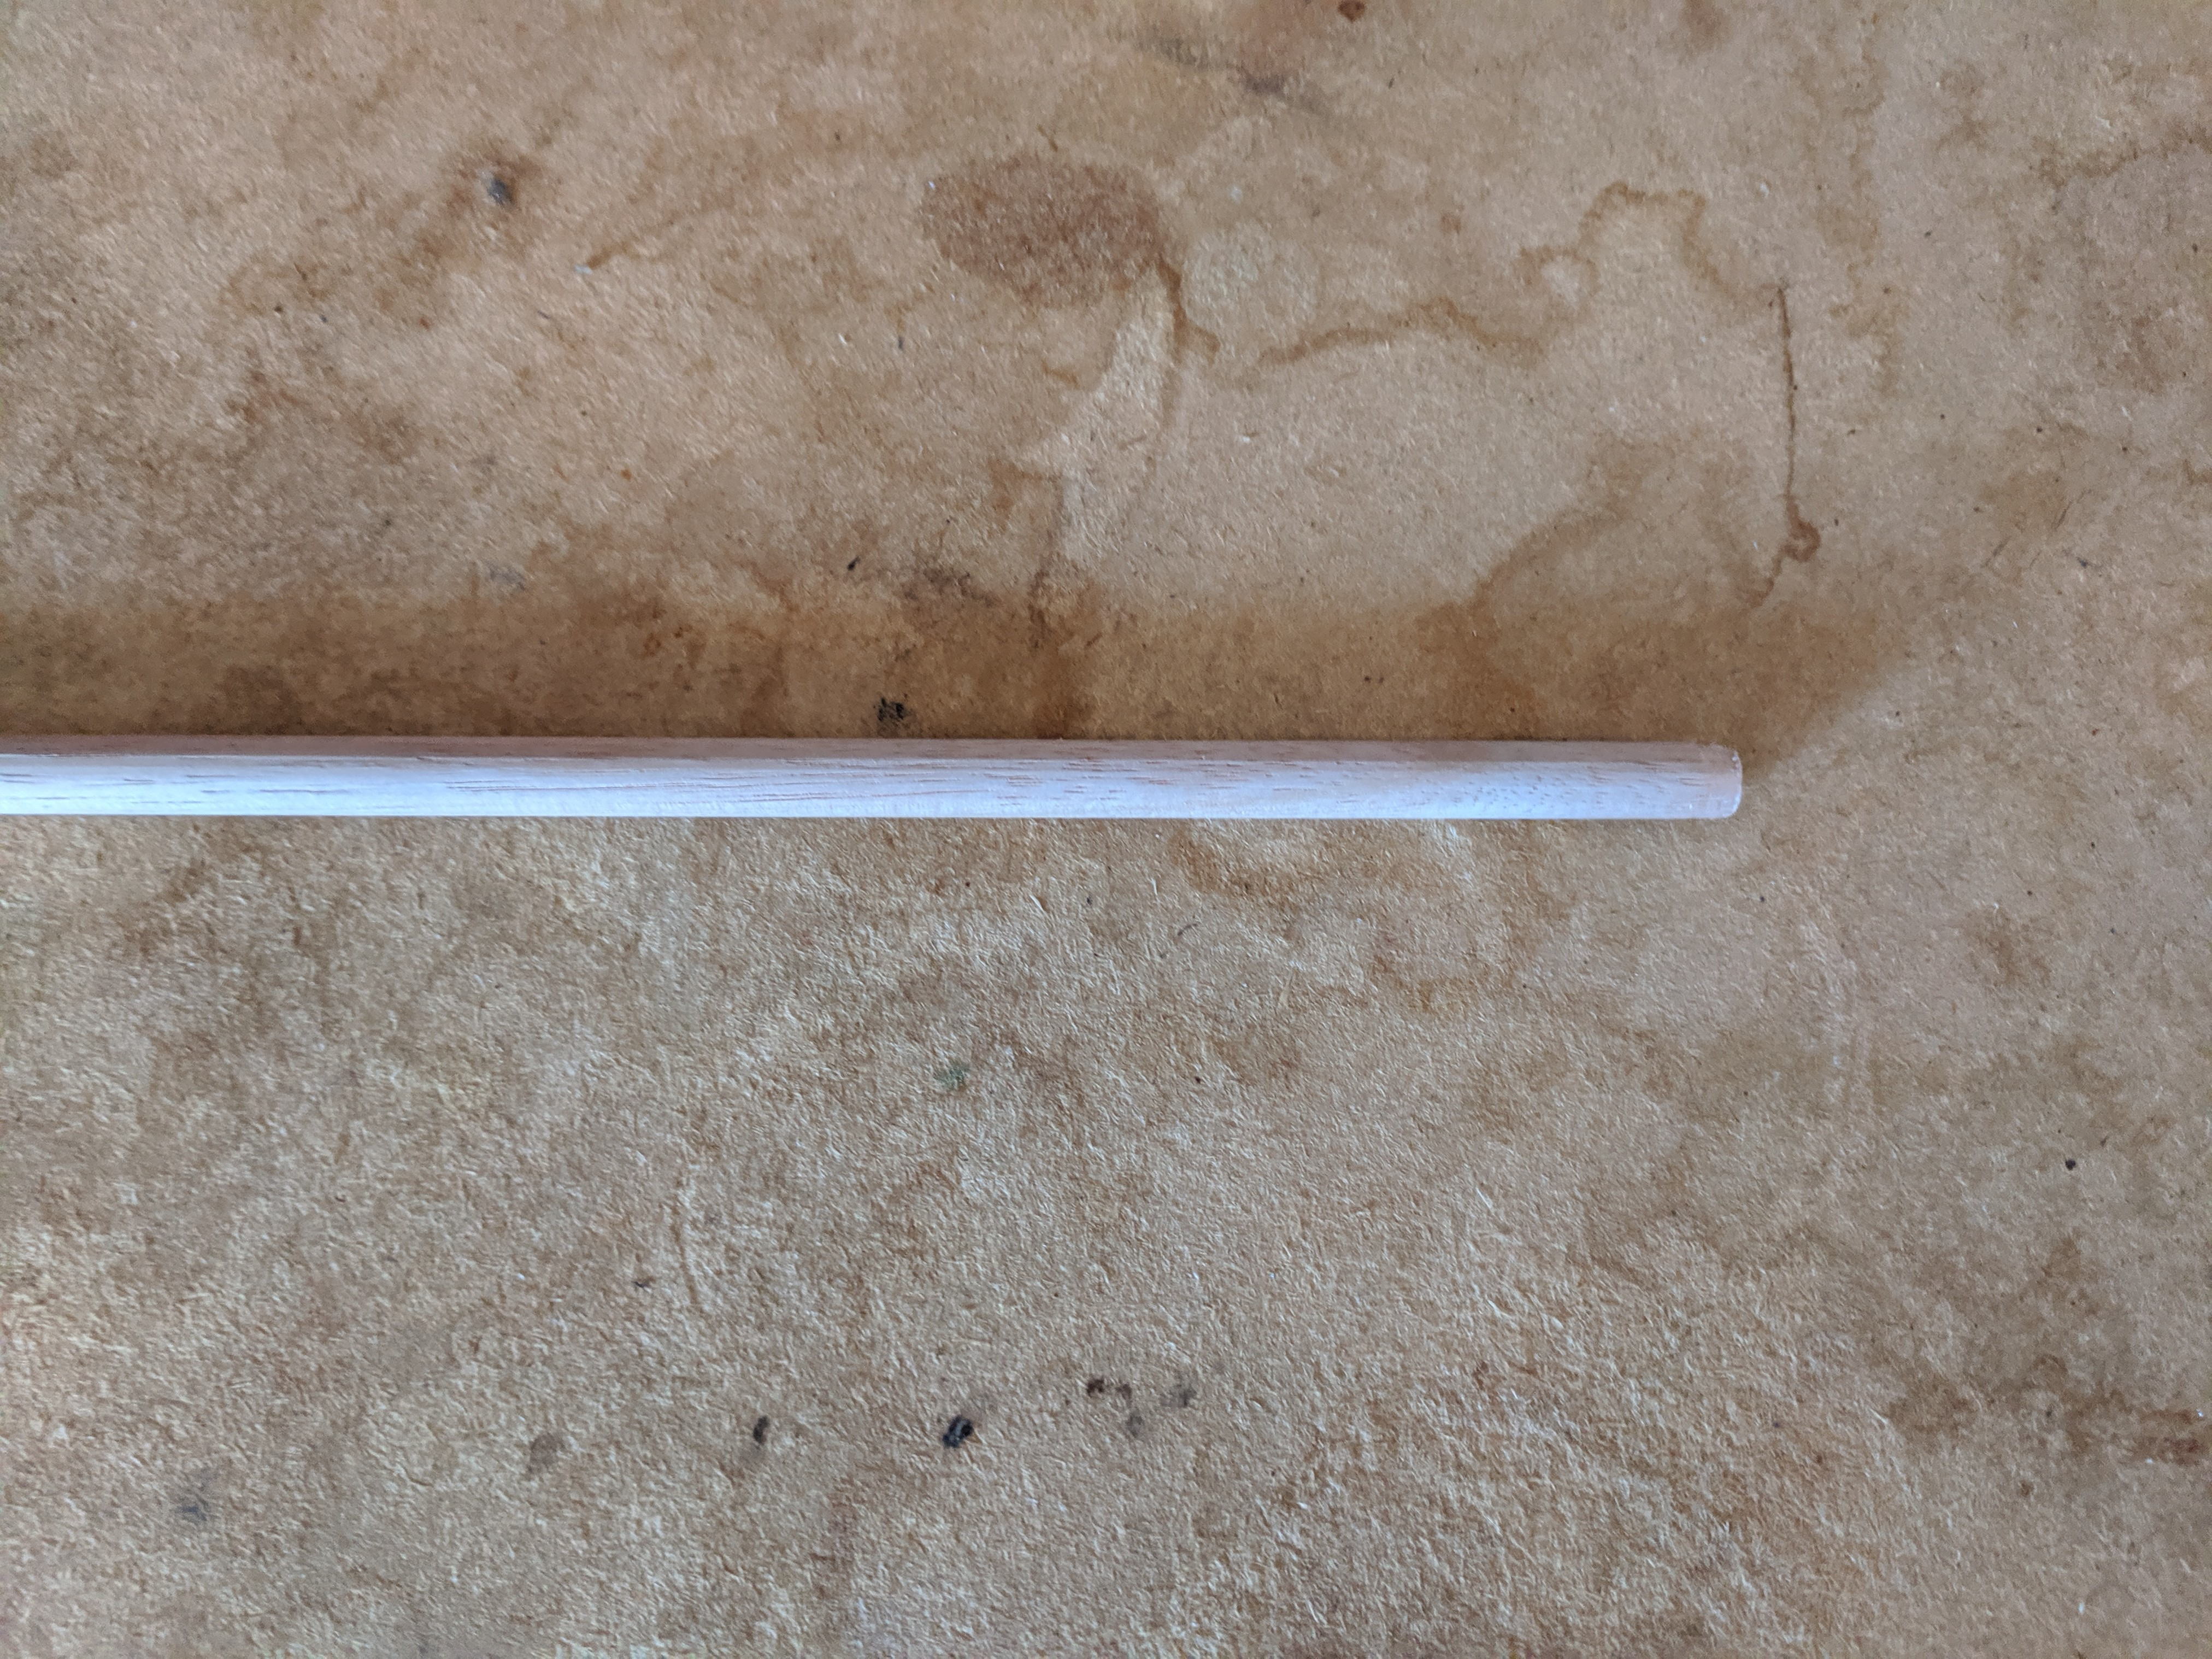
\includegraphics[height=5cm]{dowel}}
		\caption{Dowel lengths used for both the lever arm (one used), and for the shafts (two used) to which wheels were attached.}
	\end{minipage}
	\hspace{1cm}
	\begin{minipage}[t]{0.45\textwidth}
		\centering
		\begin{tabular}{p{3.5cm}rc}
			\toprule
			Measurement & Value & Unit \\
			\midrule
			Length & 0.100 & $\si{\meter}$ \\
			Width & 0.045 & $\si{\meter}$ \\
			Mass & 0.023 & $\si{\kilogram}$ \\
			 & & \\
			\bottomrule
		\end{tabular}
		
		\vspace{0.5cm}
		
		\frame{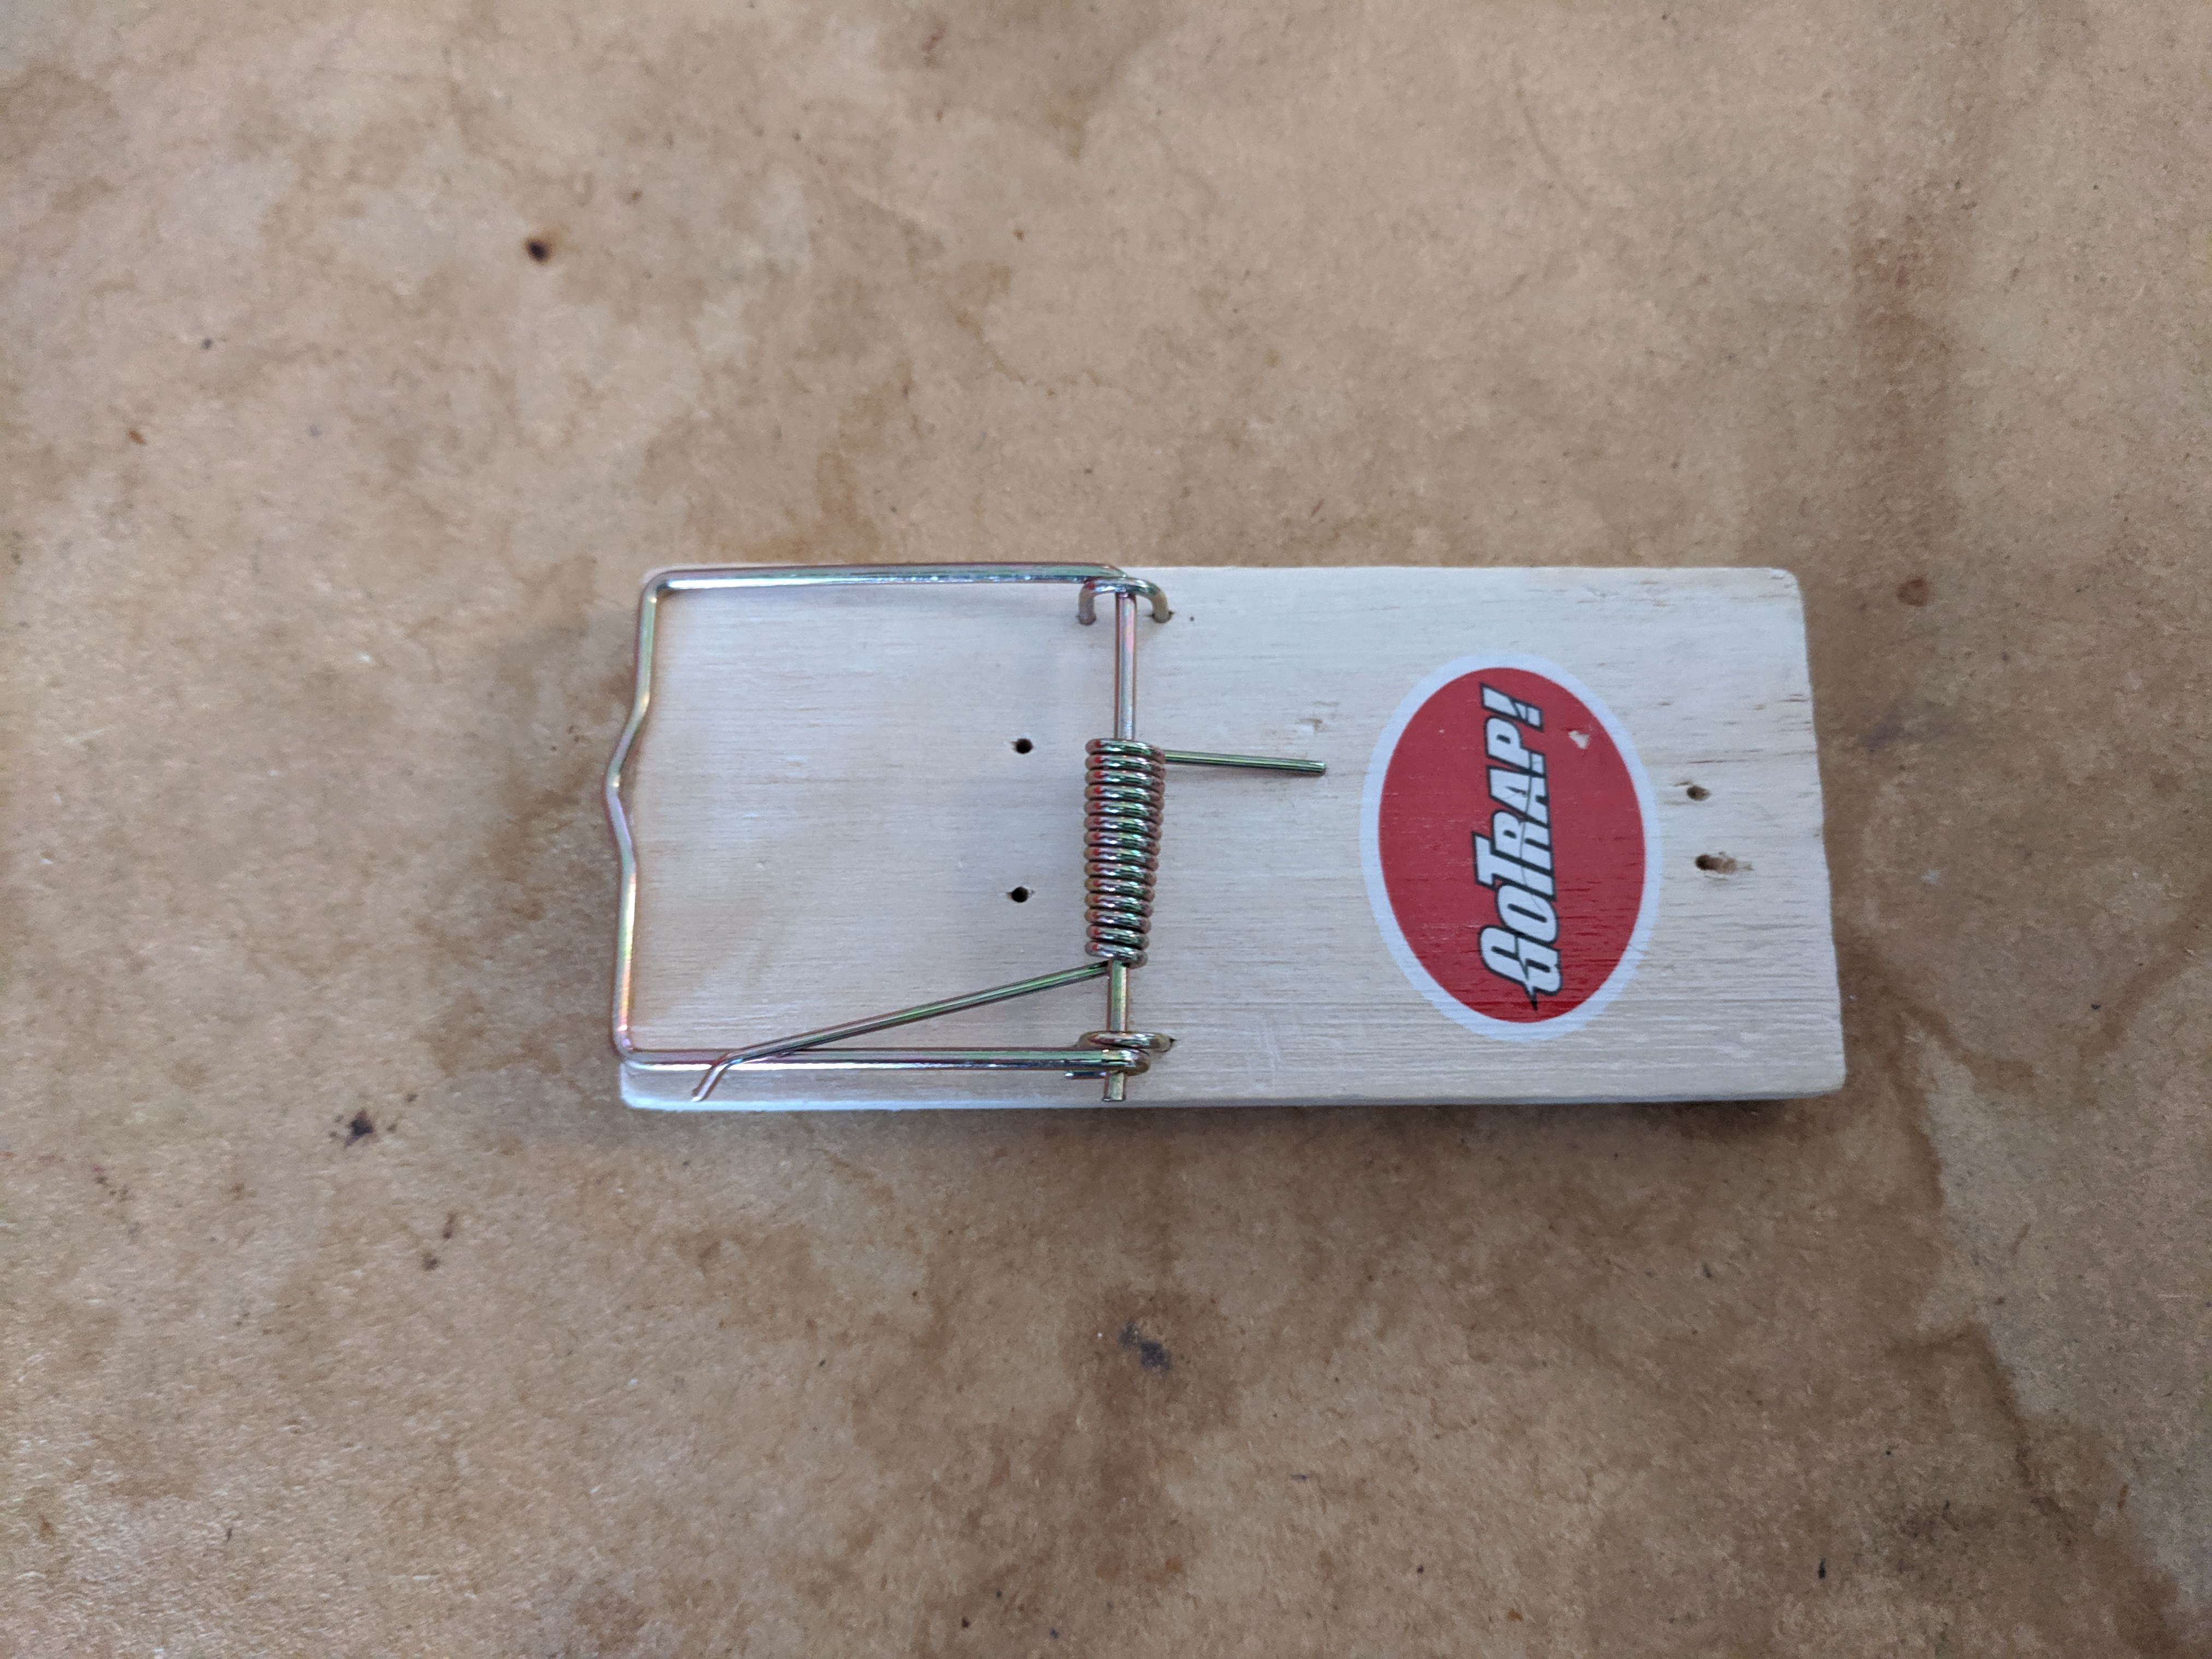
\includegraphics[height=5cm]{mouse_trap}}
		\caption{Mouse trap used to power vehicle.}
	\end{minipage}
\end{figure}

\clearpage

\section{Machine Dynamics}
\subsection{Theoretical Rolling Friction}

\subsection{Theoretical Rotational Inertia of Wheels and Shaft}

\subsection{Spring Coefficient and Potential Energy}

\subsection{title}

\section{Distance Estimation}

\section{Experimental Performance and Possible Improvements}

\section{Conclusion}

\bibliography{my_bib}
\bibliographystyle{ieeetr}

\newpage

\section{Appendix A - Datasheet}

\end{document}